\documentclass[11pt]{article}
\usepackage[textwidth=18.0cm, textheight=23.0cm, top=2.0cm]{geometry}
\usepackage{pst-all}
\usepackage{amssymb}
\usepackage{tikz}
\usepackage{underscore}\begin{document}
\pagestyle{empty}


ClassName: \underline{\textbf{Class_05.2bp-29}}
\par
BinSize: \underline{\textbf{100 × 100}}
\par
ReduceSize: \underline{\textbf{100 × 100}}
\par
TypeNum: \underline{\textbf{60}}
\par
Num: \underline{\textbf{60}}
\par
OutS: \underline{\textbf{240000}}
\par
InS: \underline{\textbf{183568}}
\par
Rate: \underline{\textbf{0.765}}
\par
UB: \underline{\textbf{24}}
\par
LB0: \underline{\textbf{23}}
\par
LB: \underline{\textbf{24}}
\par
LBWithCut: \underline{\textbf{24}}
\par
NodeCut: \underline{\textbf{0}}
\par
ExtendedNodeCnt: \underline{\textbf{1}}
\par
GenNodeCnt: \underline{\textbf{1}}
\par
PrimalNode: \underline{\textbf{0}}
\par
ColumnCount: \underline{\textbf{47}}
\par
TotalCutCount: \underline{\textbf{0}}
\par
RootCutCount: \underline{\textbf{0}}
\par
LPSolverCnt: \underline{\textbf{24}}
\par
PricingSolverCnt: \underline{\textbf{24}}
\par
BranchAndBoundNum: \underline{\textbf{1}}
\par
isOpt: \underline{\textbf{true}}
\par
TimeOnInitSolution: \underline{\textbf{0.080 s}}
\par
TimeOnPrimal: \underline{\textbf{0.000 s}}
\par
TimeOnPricing: \underline{\textbf{1.125 s}}
\par
TimeOnRmp: \underline{\textbf{0.078 s}}
\par
TotalTime: \underline{\textbf{1.330 s}}
\par
\newpage


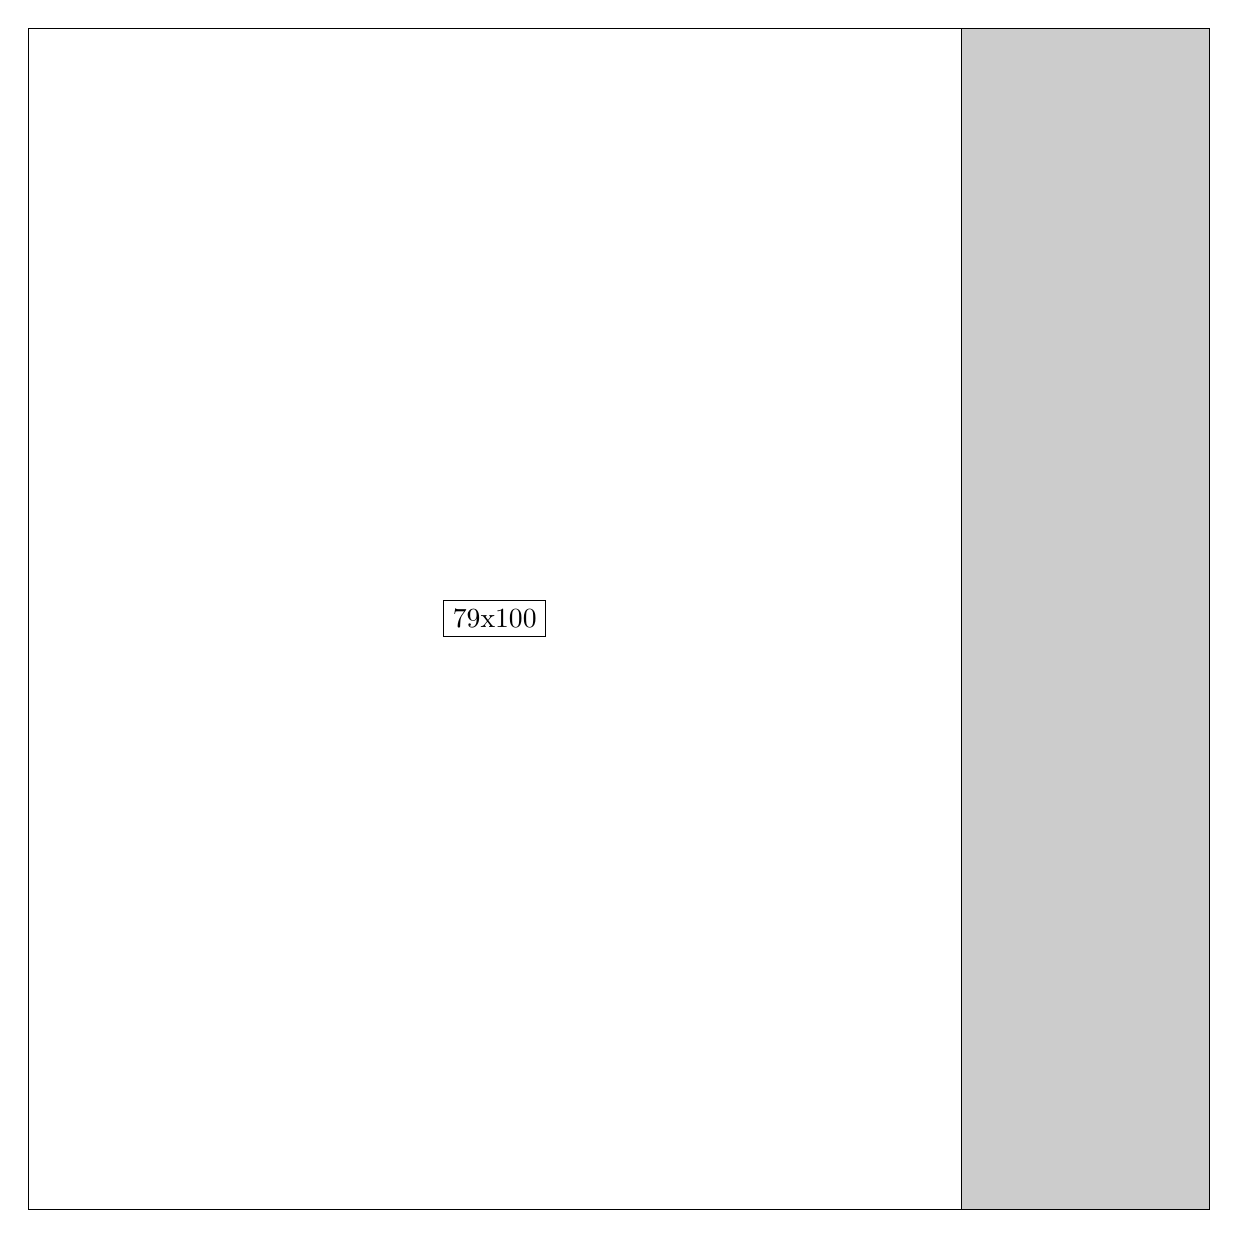
\begin{tikzpicture}[shorten >=1pt,scale=1.0,every node/.style={scale=1.0},->]
\tikzstyle{vertex}=[circle,fill=black!25,minimum size=14pt,inner sep=0pt]
\filldraw[fill=gray!40!white, draw=black] (0,0) rectangle (15.0,15.0);
\foreach \name/\x/\y/\w/\h in {79x100/0.0/0.0/11.85/15.0}
\filldraw[fill=white!40!white, draw=black] (\x,\y) rectangle node[draw] (\name) {\name} ++(\w,\h);
\end{tikzpicture}


w =79 , h =100 , x =0 , y =0 , v =7900
\par
\newpage



\begin{tikzpicture}[shorten >=1pt,scale=1.0,every node/.style={scale=1.0},->]
\tikzstyle{vertex}=[circle,fill=black!25,minimum size=14pt,inner sep=0pt]
\filldraw[fill=gray!40!white, draw=black] (0,0) rectangle (15.0,15.0);
\foreach \name/\x/\y/\w/\h in {96x78/0.0/0.0/14.399999999999999/11.7}
\filldraw[fill=white!40!white, draw=black] (\x,\y) rectangle node[draw] (\name) {\name} ++(\w,\h);
\end{tikzpicture}


w =96 , h =78 , x =0 , y =0 , v =7488
\par
\newpage


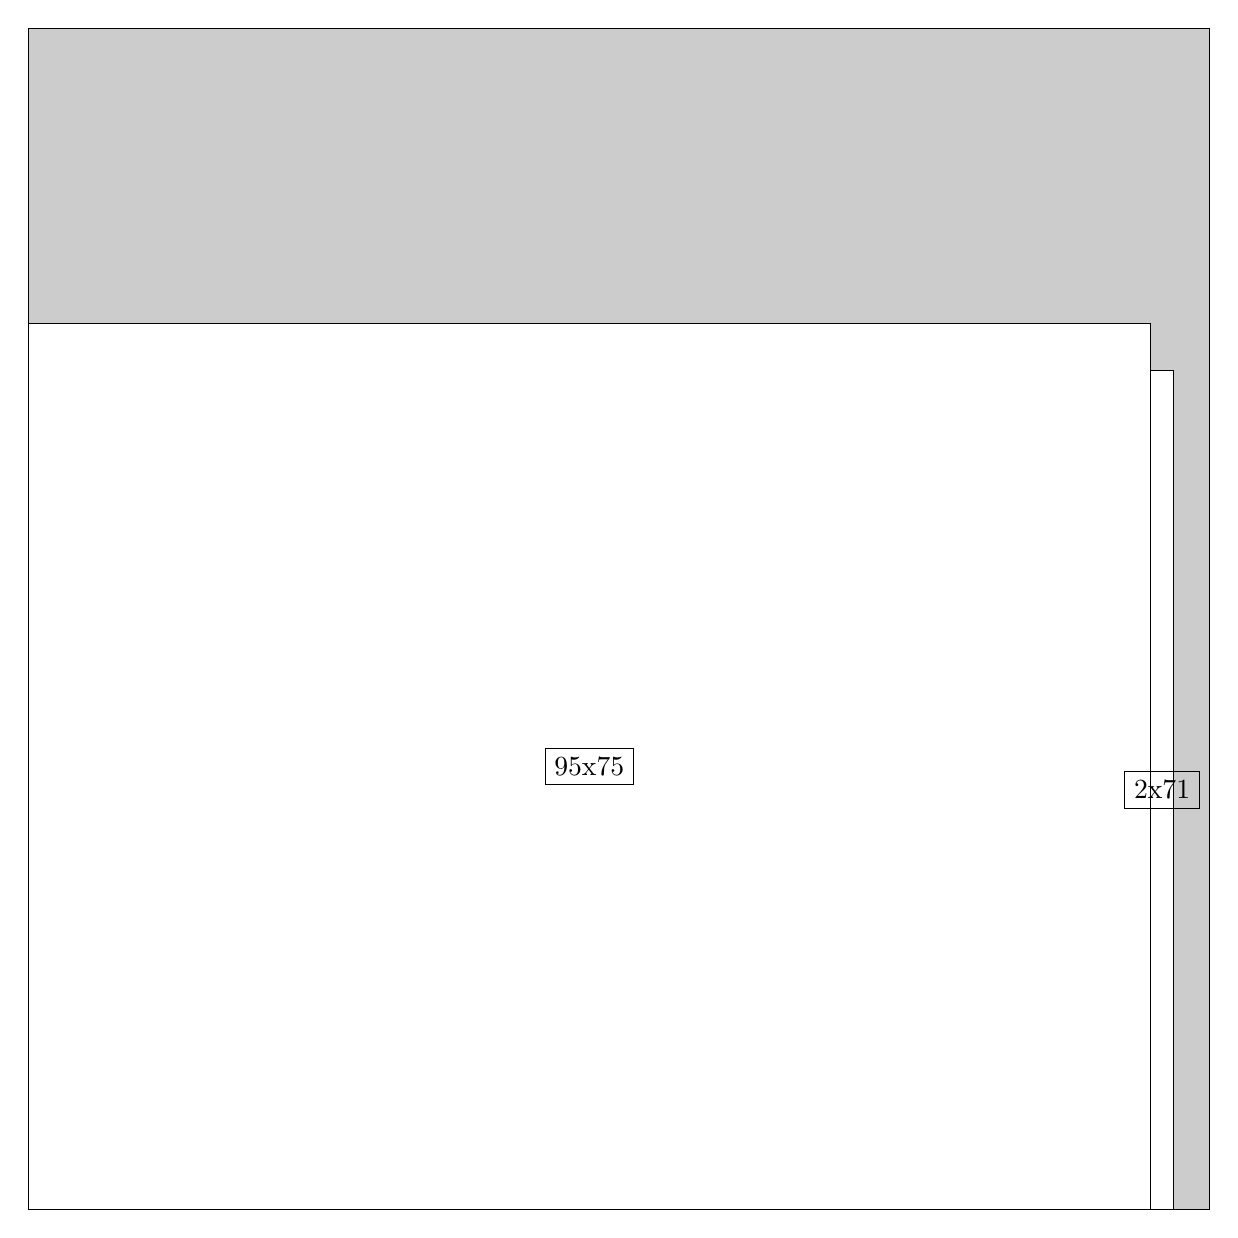
\begin{tikzpicture}[shorten >=1pt,scale=1.0,every node/.style={scale=1.0},->]
\tikzstyle{vertex}=[circle,fill=black!25,minimum size=14pt,inner sep=0pt]
\filldraw[fill=gray!40!white, draw=black] (0,0) rectangle (15.0,15.0);
\foreach \name/\x/\y/\w/\h in {95x75/0.0/0.0/14.25/11.25,2x71/14.25/0.0/0.3/10.65}
\filldraw[fill=white!40!white, draw=black] (\x,\y) rectangle node[draw] (\name) {\name} ++(\w,\h);
\end{tikzpicture}


w =95 , h =75 , x =0 , y =0 , v =7125
\par
w =2 , h =71 , x =95 , y =0 , v =142
\par
\newpage


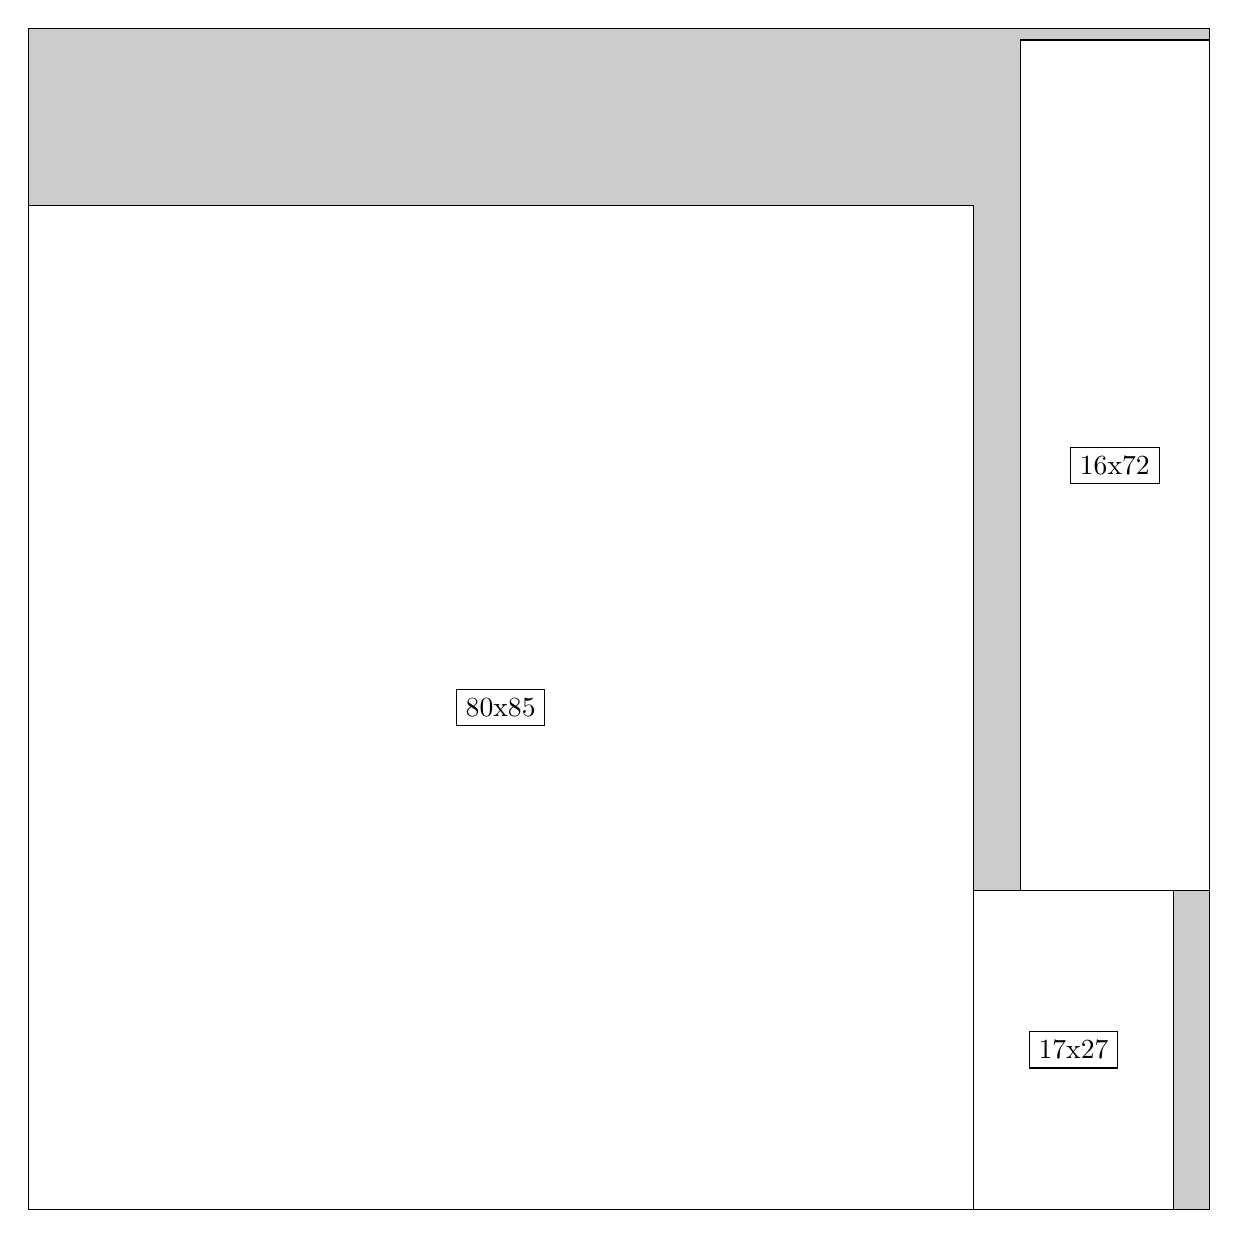
\begin{tikzpicture}[shorten >=1pt,scale=1.0,every node/.style={scale=1.0},->]
\tikzstyle{vertex}=[circle,fill=black!25,minimum size=14pt,inner sep=0pt]
\filldraw[fill=gray!40!white, draw=black] (0,0) rectangle (15.0,15.0);
\foreach \name/\x/\y/\w/\h in {80x85/0.0/0.0/12.0/12.75,16x72/12.6/4.05/2.4/10.799999999999999,17x27/12.0/0.0/2.55/4.05}
\filldraw[fill=white!40!white, draw=black] (\x,\y) rectangle node[draw] (\name) {\name} ++(\w,\h);
\end{tikzpicture}


w =80 , h =85 , x =0 , y =0 , v =6800
\par
w =16 , h =72 , x =84 , y =27 , v =1152
\par
w =17 , h =27 , x =80 , y =0 , v =459
\par
\newpage


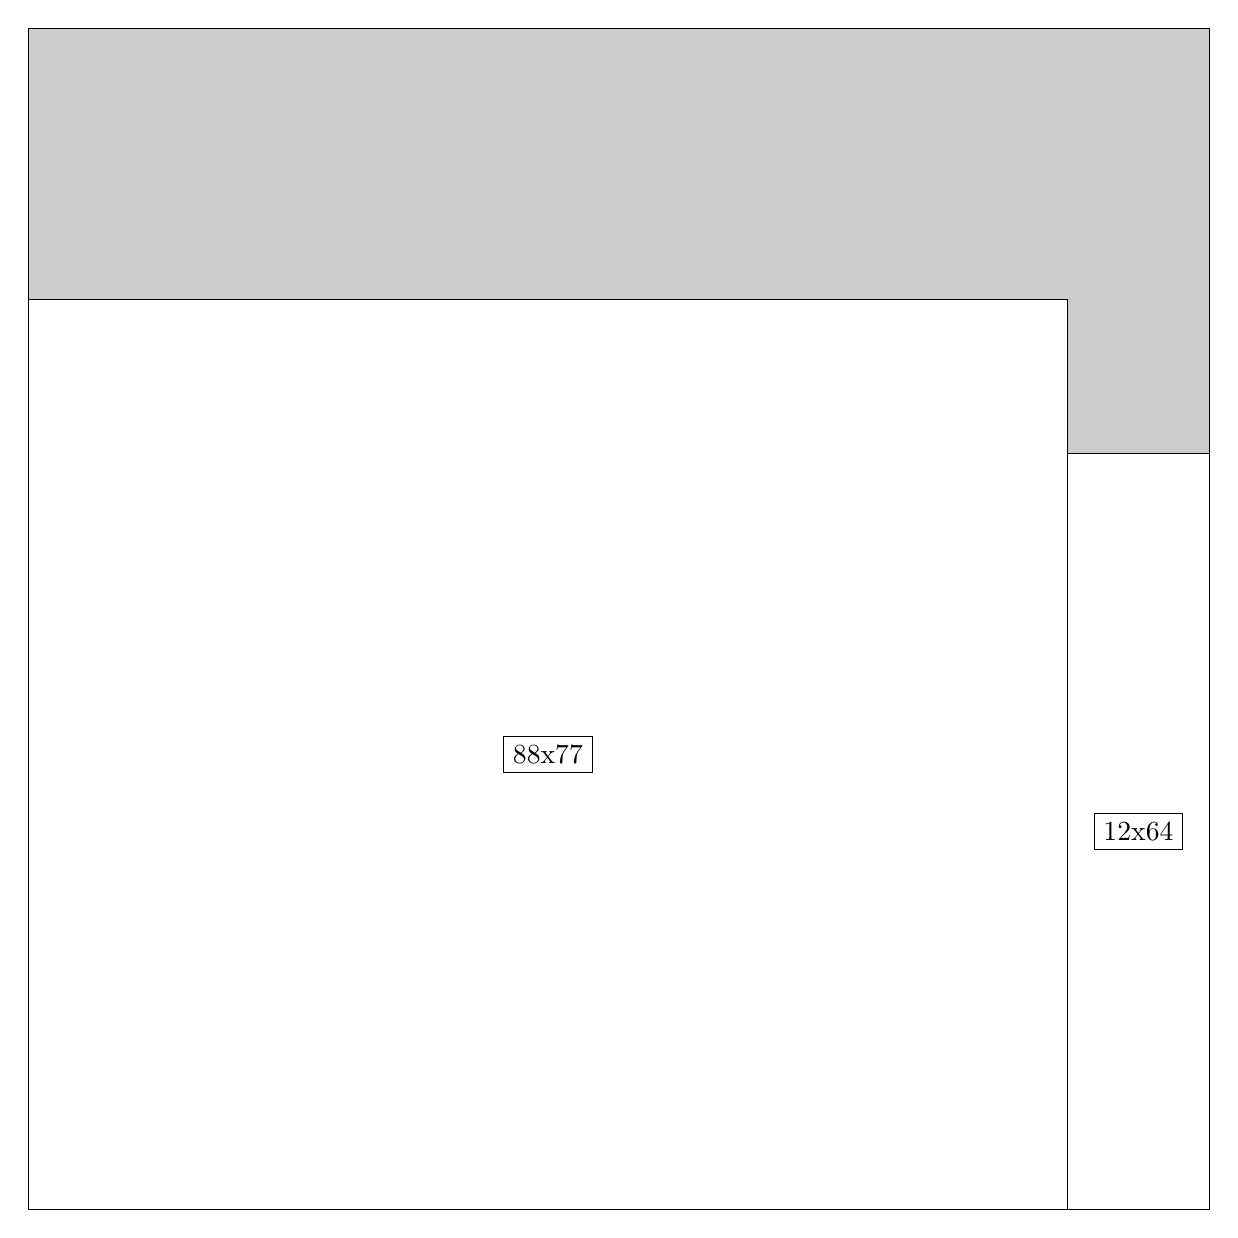
\begin{tikzpicture}[shorten >=1pt,scale=1.0,every node/.style={scale=1.0},->]
\tikzstyle{vertex}=[circle,fill=black!25,minimum size=14pt,inner sep=0pt]
\filldraw[fill=gray!40!white, draw=black] (0,0) rectangle (15.0,15.0);
\foreach \name/\x/\y/\w/\h in {88x77/0.0/0.0/13.2/11.549999999999999,12x64/13.2/0.0/1.7999999999999998/9.6}
\filldraw[fill=white!40!white, draw=black] (\x,\y) rectangle node[draw] (\name) {\name} ++(\w,\h);
\end{tikzpicture}


w =88 , h =77 , x =0 , y =0 , v =6776
\par
w =12 , h =64 , x =88 , y =0 , v =768
\par
\newpage


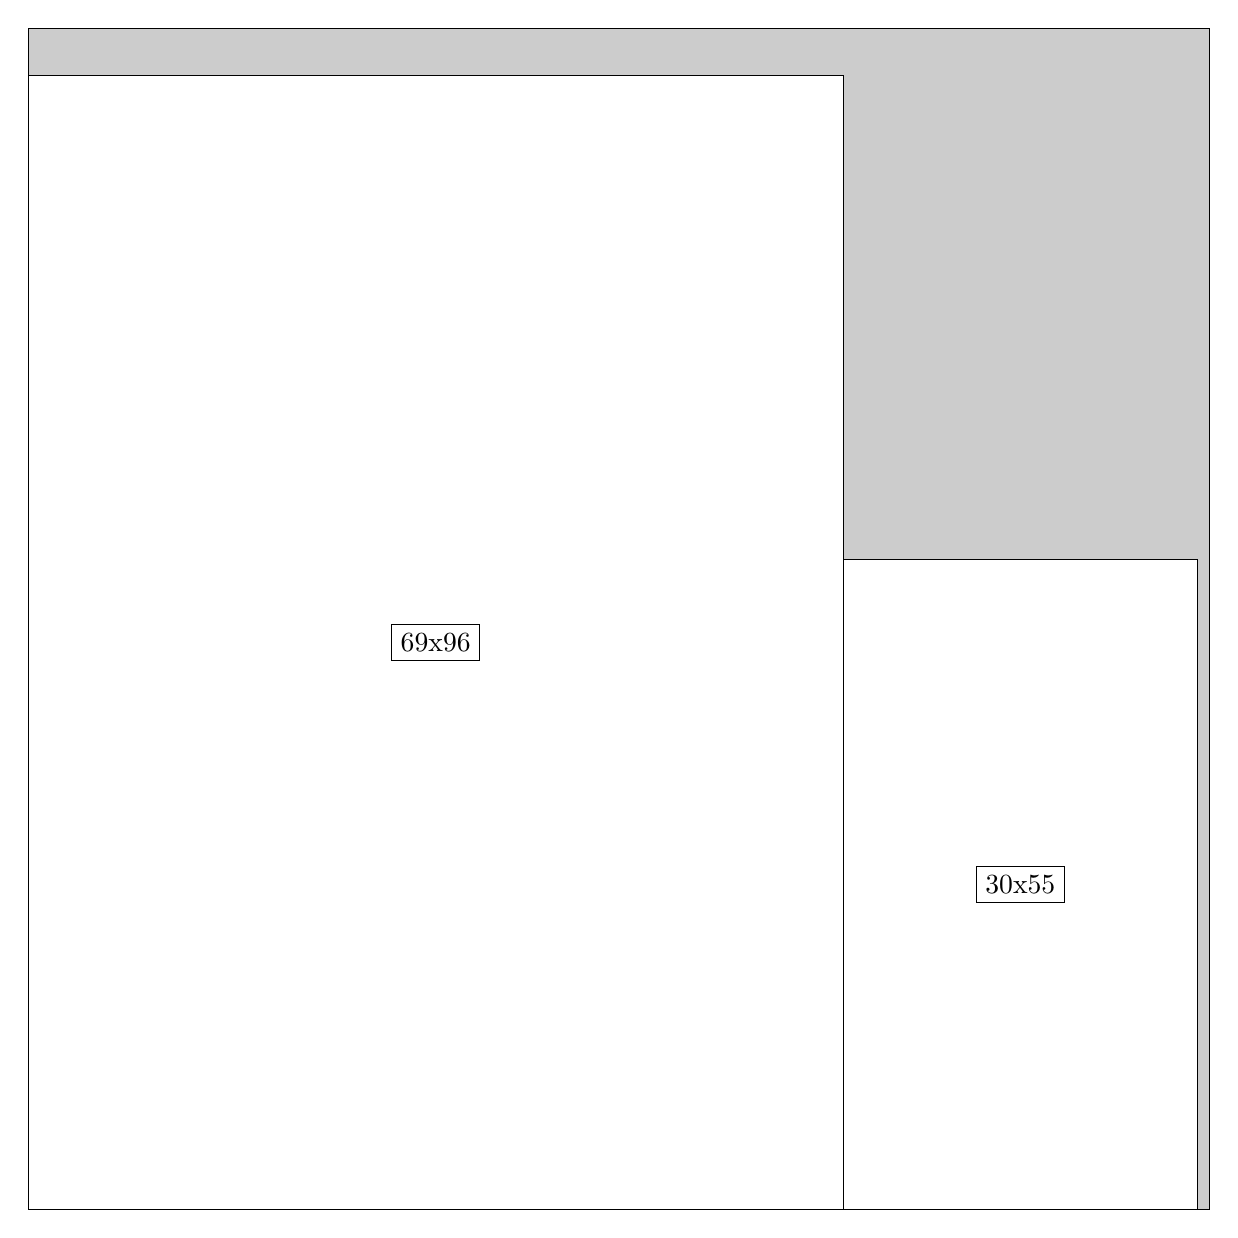
\begin{tikzpicture}[shorten >=1pt,scale=1.0,every node/.style={scale=1.0},->]
\tikzstyle{vertex}=[circle,fill=black!25,minimum size=14pt,inner sep=0pt]
\filldraw[fill=gray!40!white, draw=black] (0,0) rectangle (15.0,15.0);
\foreach \name/\x/\y/\w/\h in {69x96/0.0/0.0/10.35/14.399999999999999,30x55/10.35/0.0/4.5/8.25}
\filldraw[fill=white!40!white, draw=black] (\x,\y) rectangle node[draw] (\name) {\name} ++(\w,\h);
\end{tikzpicture}


w =69 , h =96 , x =0 , y =0 , v =6624
\par
w =30 , h =55 , x =69 , y =0 , v =1650
\par
\newpage


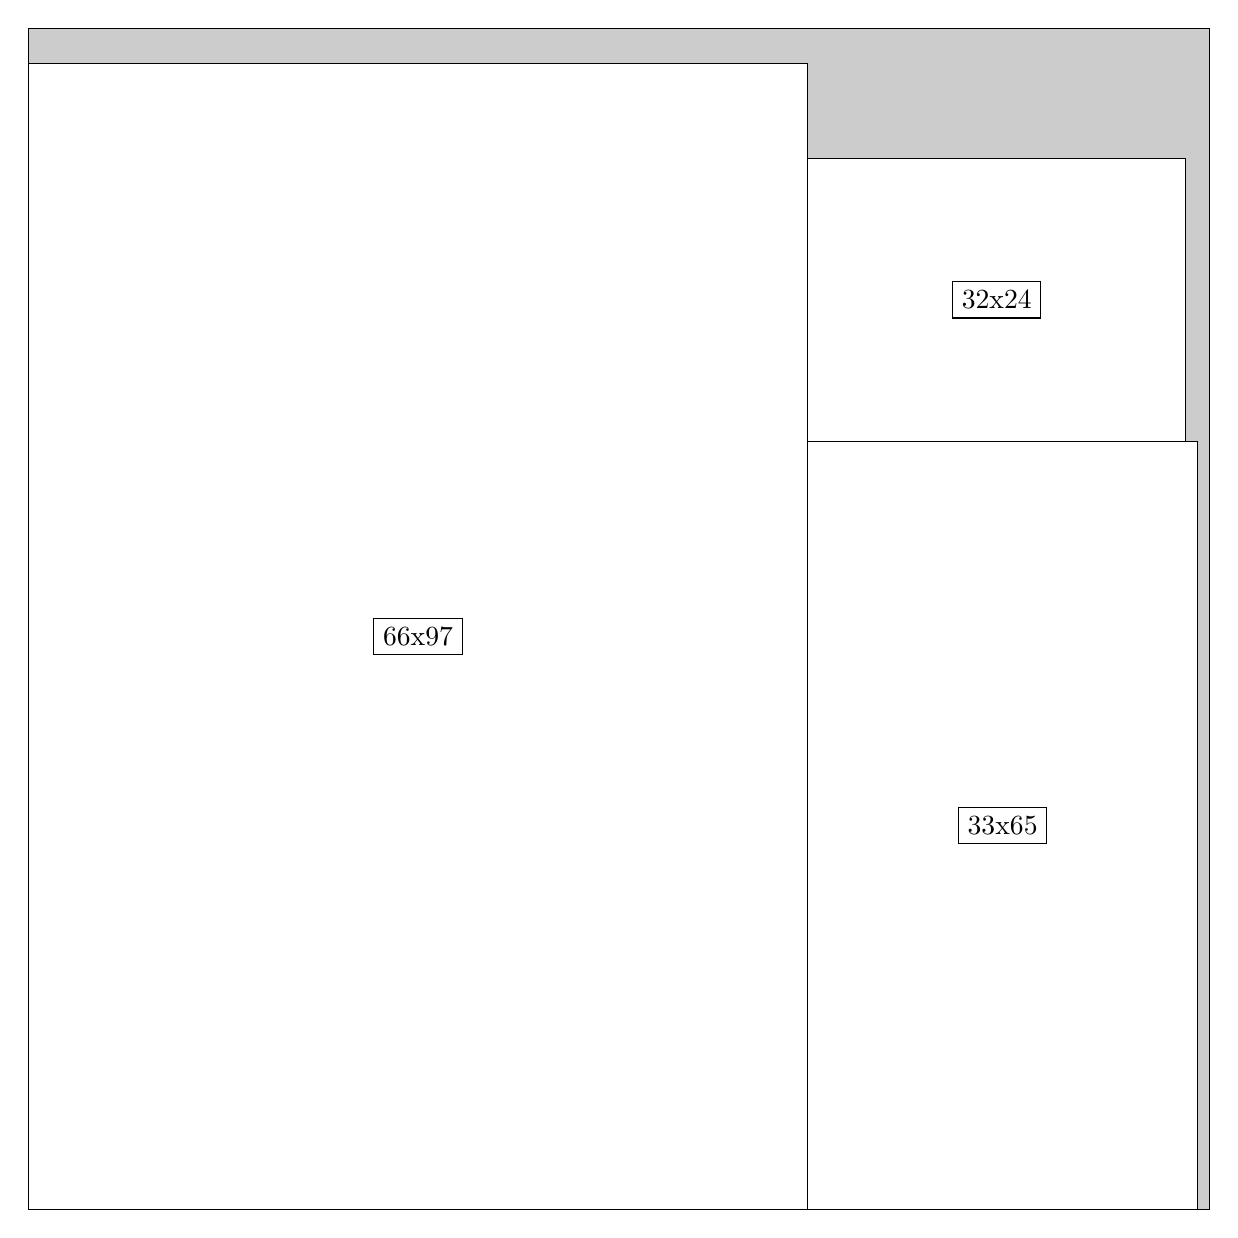
\begin{tikzpicture}[shorten >=1pt,scale=1.0,every node/.style={scale=1.0},->]
\tikzstyle{vertex}=[circle,fill=black!25,minimum size=14pt,inner sep=0pt]
\filldraw[fill=gray!40!white, draw=black] (0,0) rectangle (15.0,15.0);
\foreach \name/\x/\y/\w/\h in {66x97/0.0/0.0/9.9/14.549999999999999,33x65/9.9/0.0/4.95/9.75,32x24/9.9/9.75/4.8/3.5999999999999996}
\filldraw[fill=white!40!white, draw=black] (\x,\y) rectangle node[draw] (\name) {\name} ++(\w,\h);
\end{tikzpicture}


w =66 , h =97 , x =0 , y =0 , v =6402
\par
w =33 , h =65 , x =66 , y =0 , v =2145
\par
w =32 , h =24 , x =66 , y =65 , v =768
\par
\newpage


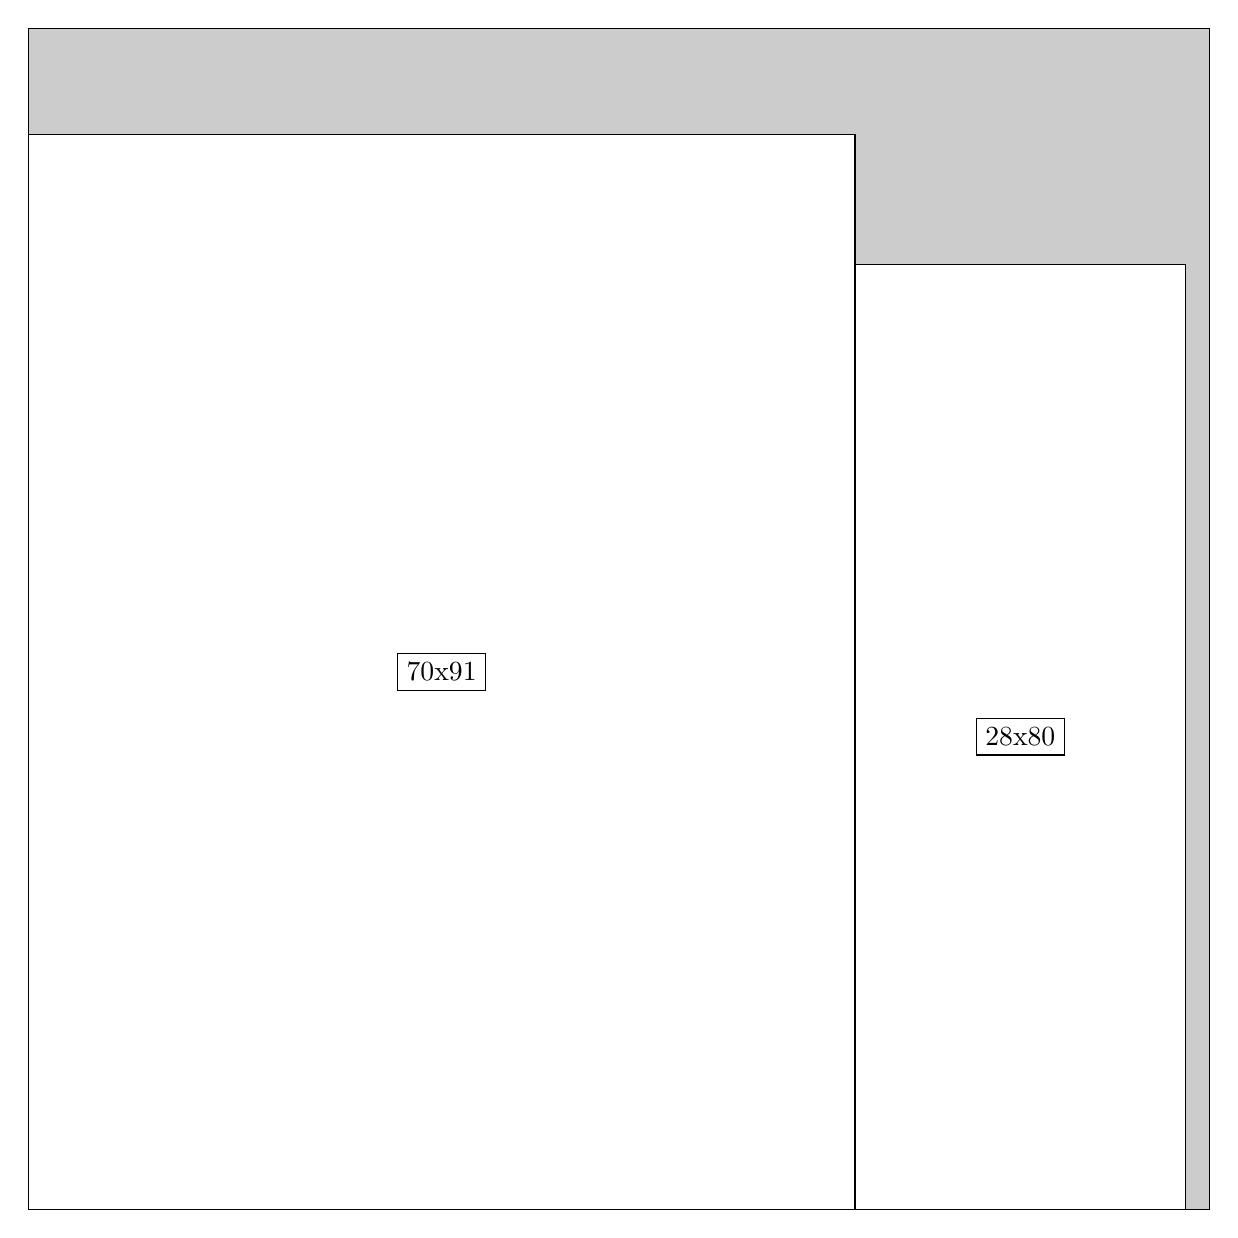
\begin{tikzpicture}[shorten >=1pt,scale=1.0,every node/.style={scale=1.0},->]
\tikzstyle{vertex}=[circle,fill=black!25,minimum size=14pt,inner sep=0pt]
\filldraw[fill=gray!40!white, draw=black] (0,0) rectangle (15.0,15.0);
\foreach \name/\x/\y/\w/\h in {70x91/0.0/0.0/10.5/13.65,28x80/10.5/0.0/4.2/12.0}
\filldraw[fill=white!40!white, draw=black] (\x,\y) rectangle node[draw] (\name) {\name} ++(\w,\h);
\end{tikzpicture}


w =70 , h =91 , x =0 , y =0 , v =6370
\par
w =28 , h =80 , x =70 , y =0 , v =2240
\par
\newpage


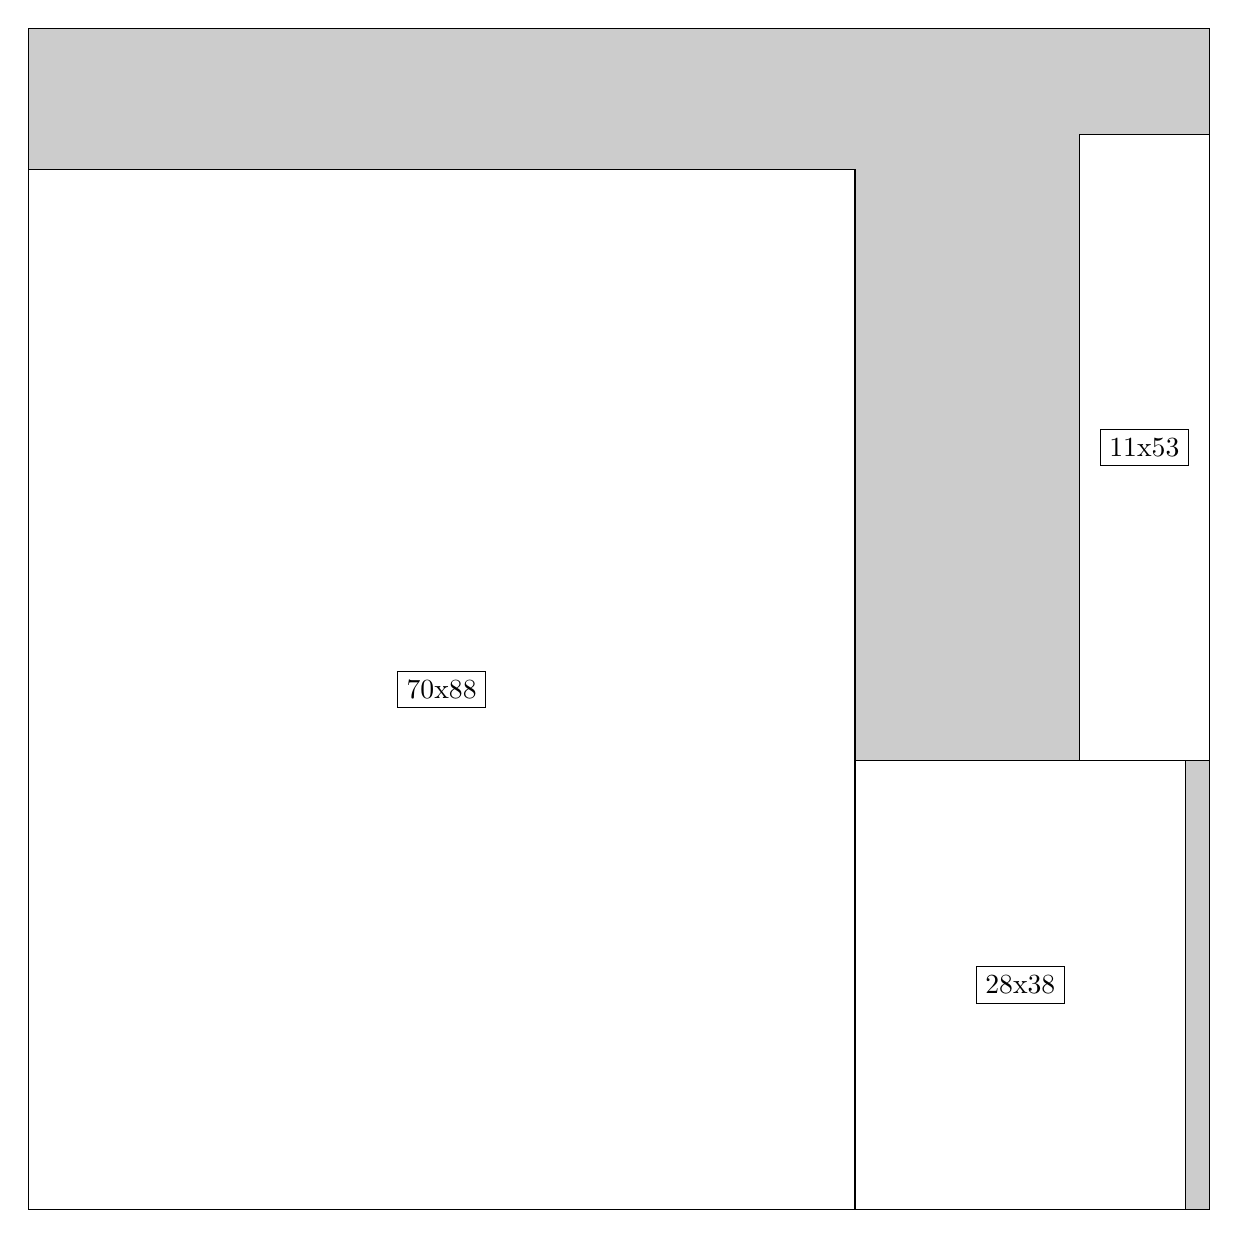
\begin{tikzpicture}[shorten >=1pt,scale=1.0,every node/.style={scale=1.0},->]
\tikzstyle{vertex}=[circle,fill=black!25,minimum size=14pt,inner sep=0pt]
\filldraw[fill=gray!40!white, draw=black] (0,0) rectangle (15.0,15.0);
\foreach \name/\x/\y/\w/\h in {70x88/0.0/0.0/10.5/13.2,28x38/10.5/0.0/4.2/5.7,11x53/13.35/5.7/1.65/7.949999999999999}
\filldraw[fill=white!40!white, draw=black] (\x,\y) rectangle node[draw] (\name) {\name} ++(\w,\h);
\end{tikzpicture}


w =70 , h =88 , x =0 , y =0 , v =6160
\par
w =28 , h =38 , x =70 , y =0 , v =1064
\par
w =11 , h =53 , x =89 , y =38 , v =583
\par
\newpage


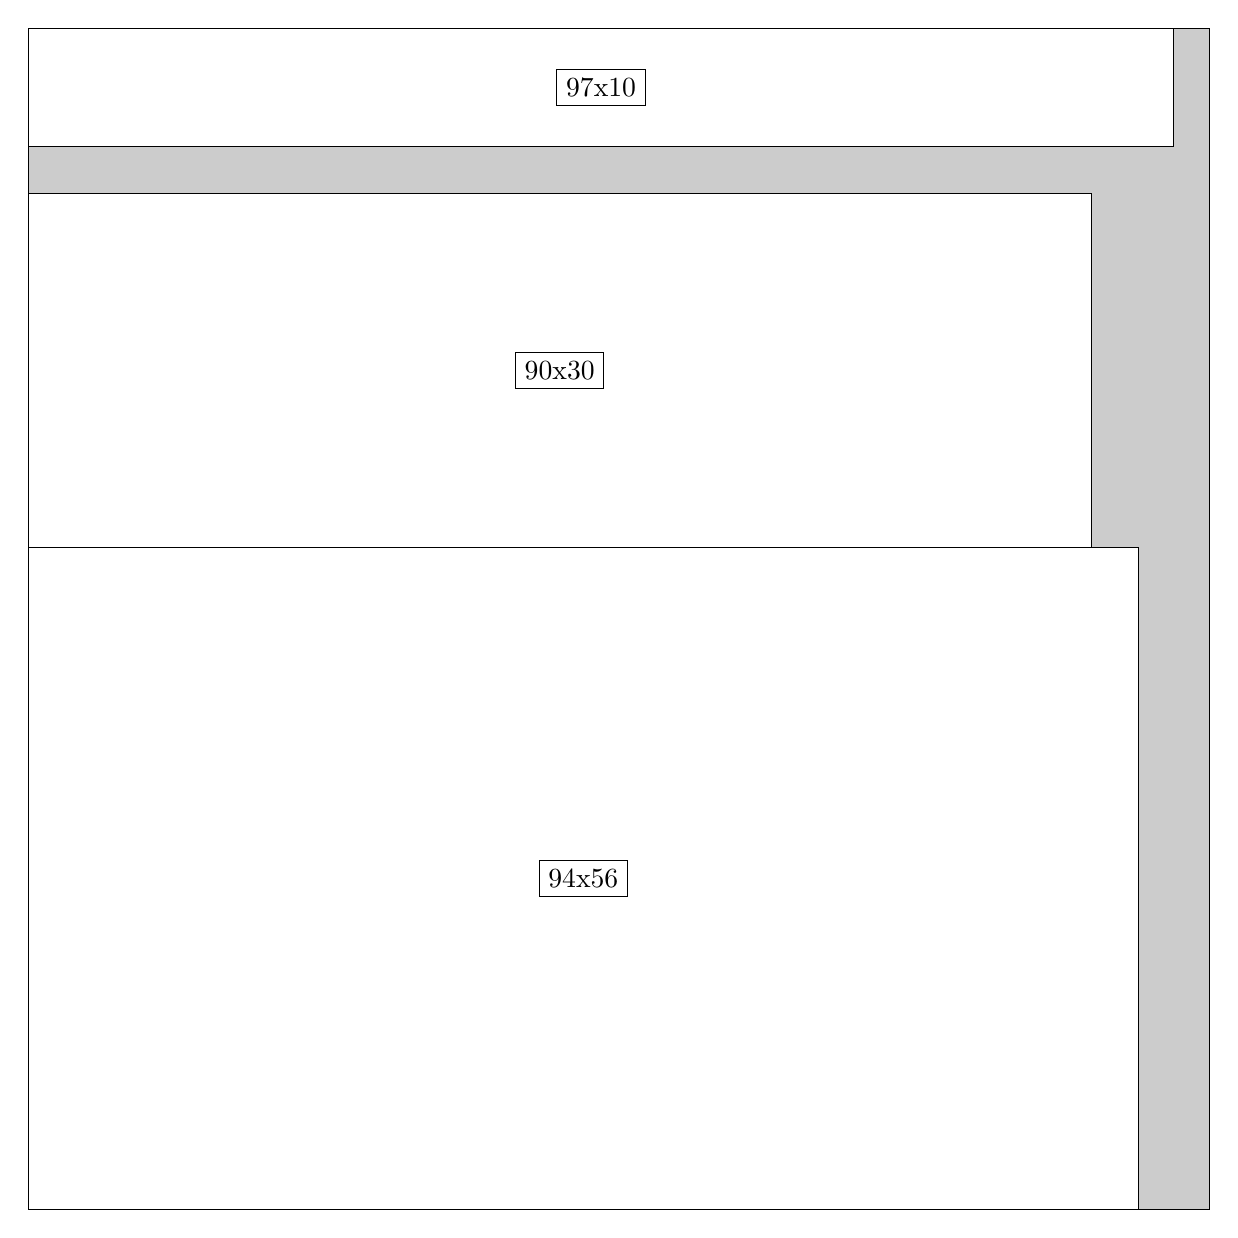
\begin{tikzpicture}[shorten >=1pt,scale=1.0,every node/.style={scale=1.0},->]
\tikzstyle{vertex}=[circle,fill=black!25,minimum size=14pt,inner sep=0pt]
\filldraw[fill=gray!40!white, draw=black] (0,0) rectangle (15.0,15.0);
\foreach \name/\x/\y/\w/\h in {94x56/0.0/0.0/14.1/8.4,90x30/0.0/8.4/13.5/4.5,97x10/0.0/13.5/14.549999999999999/1.5}
\filldraw[fill=white!40!white, draw=black] (\x,\y) rectangle node[draw] (\name) {\name} ++(\w,\h);
\end{tikzpicture}


w =94 , h =56 , x =0 , y =0 , v =5264
\par
w =90 , h =30 , x =0 , y =56 , v =2700
\par
w =97 , h =10 , x =0 , y =90 , v =970
\par
\newpage


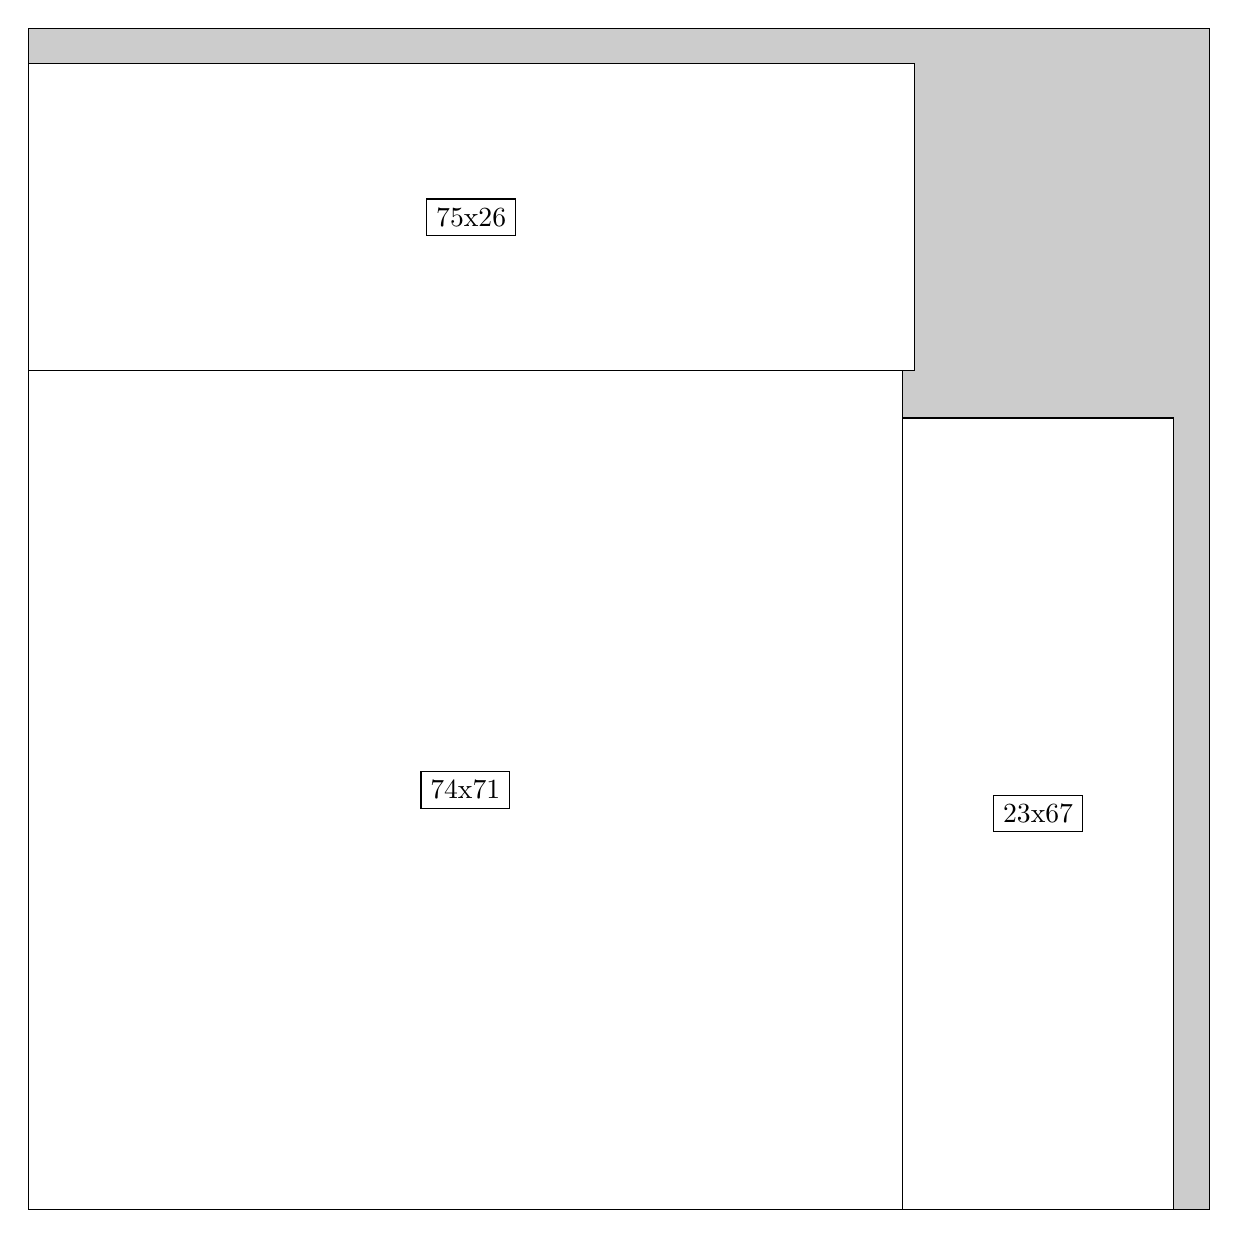
\begin{tikzpicture}[shorten >=1pt,scale=1.0,every node/.style={scale=1.0},->]
\tikzstyle{vertex}=[circle,fill=black!25,minimum size=14pt,inner sep=0pt]
\filldraw[fill=gray!40!white, draw=black] (0,0) rectangle (15.0,15.0);
\foreach \name/\x/\y/\w/\h in {74x71/0.0/0.0/11.1/10.65,75x26/0.0/10.65/11.25/3.9,23x67/11.1/0.0/3.4499999999999997/10.049999999999999}
\filldraw[fill=white!40!white, draw=black] (\x,\y) rectangle node[draw] (\name) {\name} ++(\w,\h);
\end{tikzpicture}


w =74 , h =71 , x =0 , y =0 , v =5254
\par
w =75 , h =26 , x =0 , y =71 , v =1950
\par
w =23 , h =67 , x =74 , y =0 , v =1541
\par
\newpage


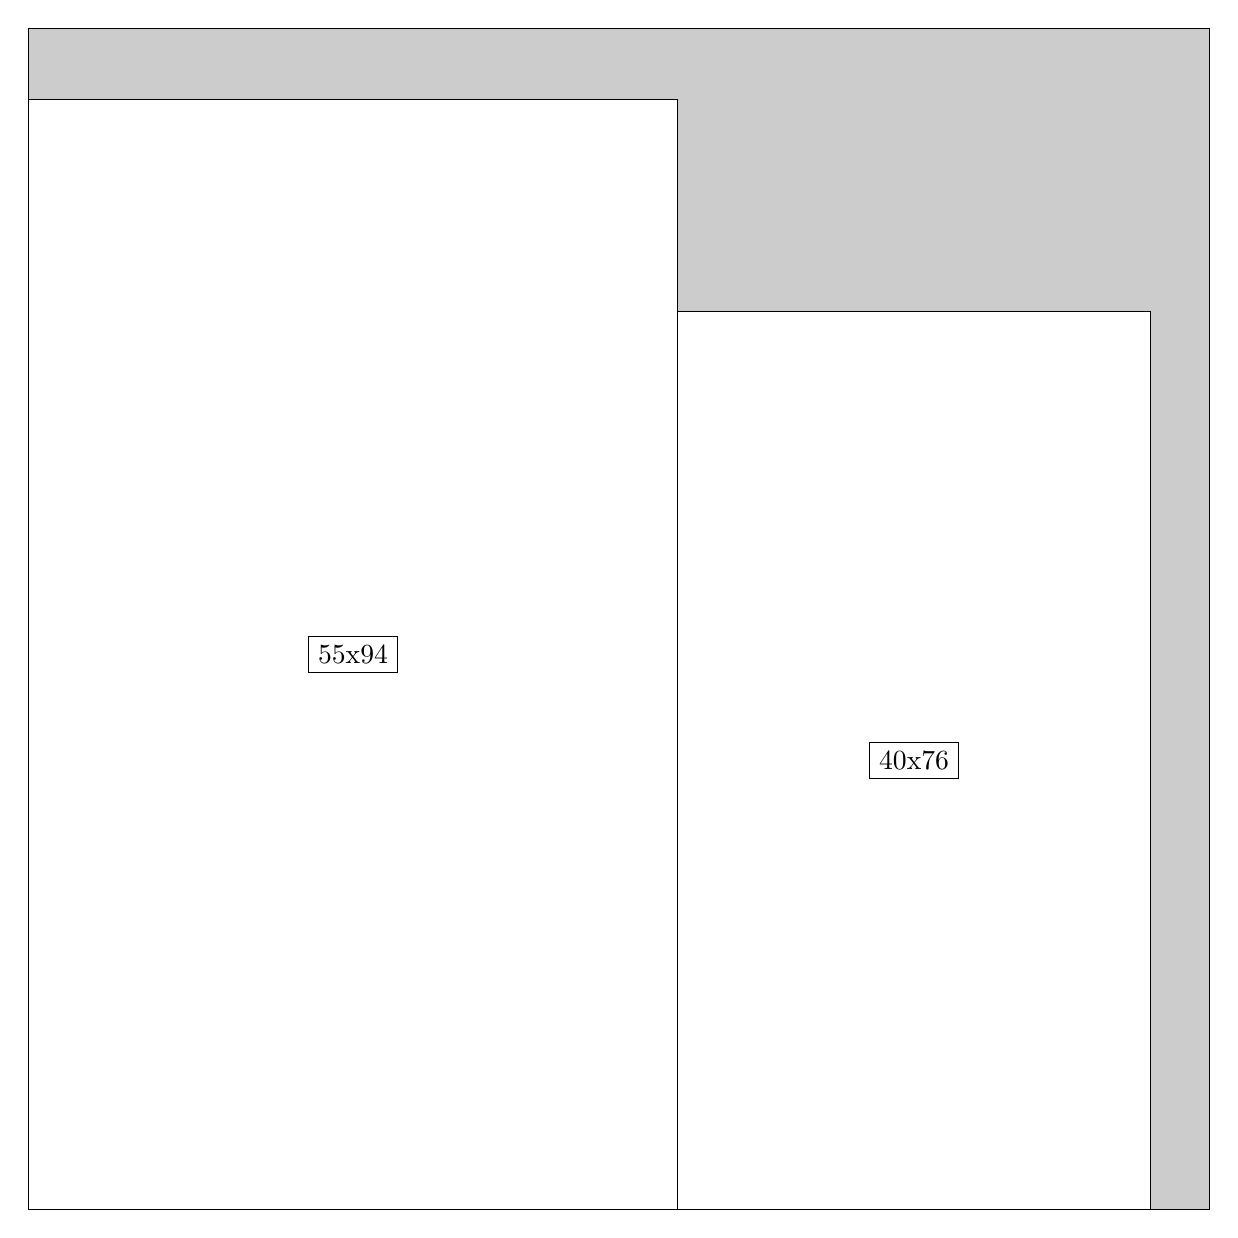
\begin{tikzpicture}[shorten >=1pt,scale=1.0,every node/.style={scale=1.0},->]
\tikzstyle{vertex}=[circle,fill=black!25,minimum size=14pt,inner sep=0pt]
\filldraw[fill=gray!40!white, draw=black] (0,0) rectangle (15.0,15.0);
\foreach \name/\x/\y/\w/\h in {55x94/0.0/0.0/8.25/14.1,40x76/8.25/0.0/6.0/11.4}
\filldraw[fill=white!40!white, draw=black] (\x,\y) rectangle node[draw] (\name) {\name} ++(\w,\h);
\end{tikzpicture}


w =55 , h =94 , x =0 , y =0 , v =5170
\par
w =40 , h =76 , x =55 , y =0 , v =3040
\par
\newpage


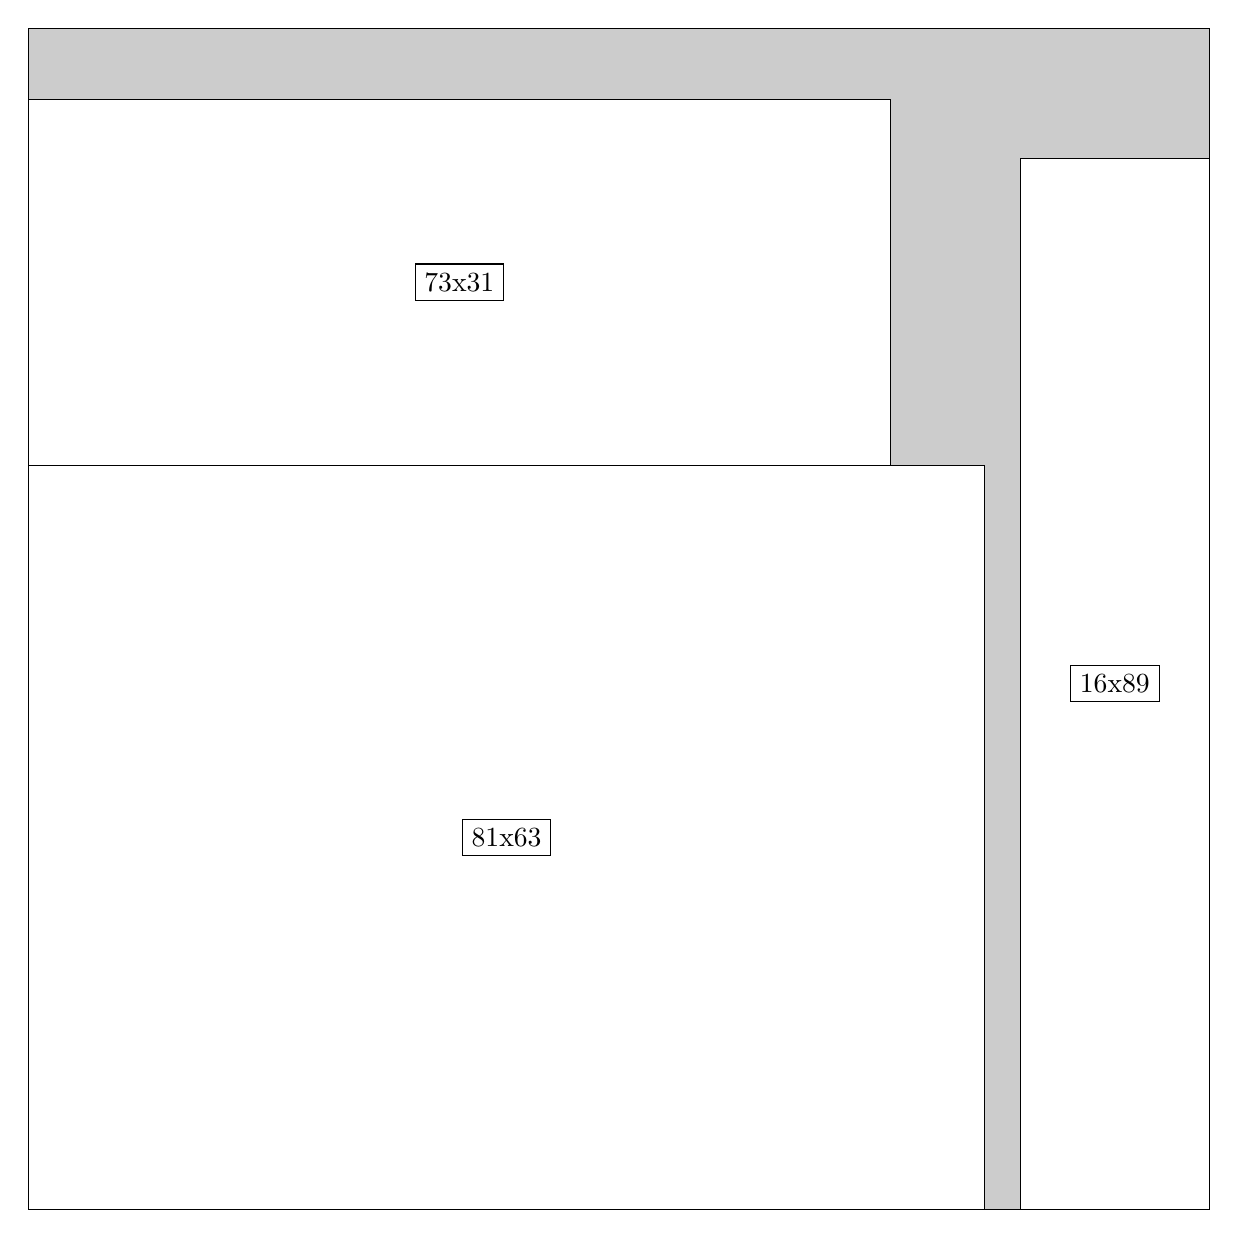
\begin{tikzpicture}[shorten >=1pt,scale=1.0,every node/.style={scale=1.0},->]
\tikzstyle{vertex}=[circle,fill=black!25,minimum size=14pt,inner sep=0pt]
\filldraw[fill=gray!40!white, draw=black] (0,0) rectangle (15.0,15.0);
\foreach \name/\x/\y/\w/\h in {81x63/0.0/0.0/12.15/9.45,73x31/0.0/9.45/10.95/4.6499999999999995,16x89/12.6/0.0/2.4/13.35}
\filldraw[fill=white!40!white, draw=black] (\x,\y) rectangle node[draw] (\name) {\name} ++(\w,\h);
\end{tikzpicture}


w =81 , h =63 , x =0 , y =0 , v =5103
\par
w =73 , h =31 , x =0 , y =63 , v =2263
\par
w =16 , h =89 , x =84 , y =0 , v =1424
\par
\newpage


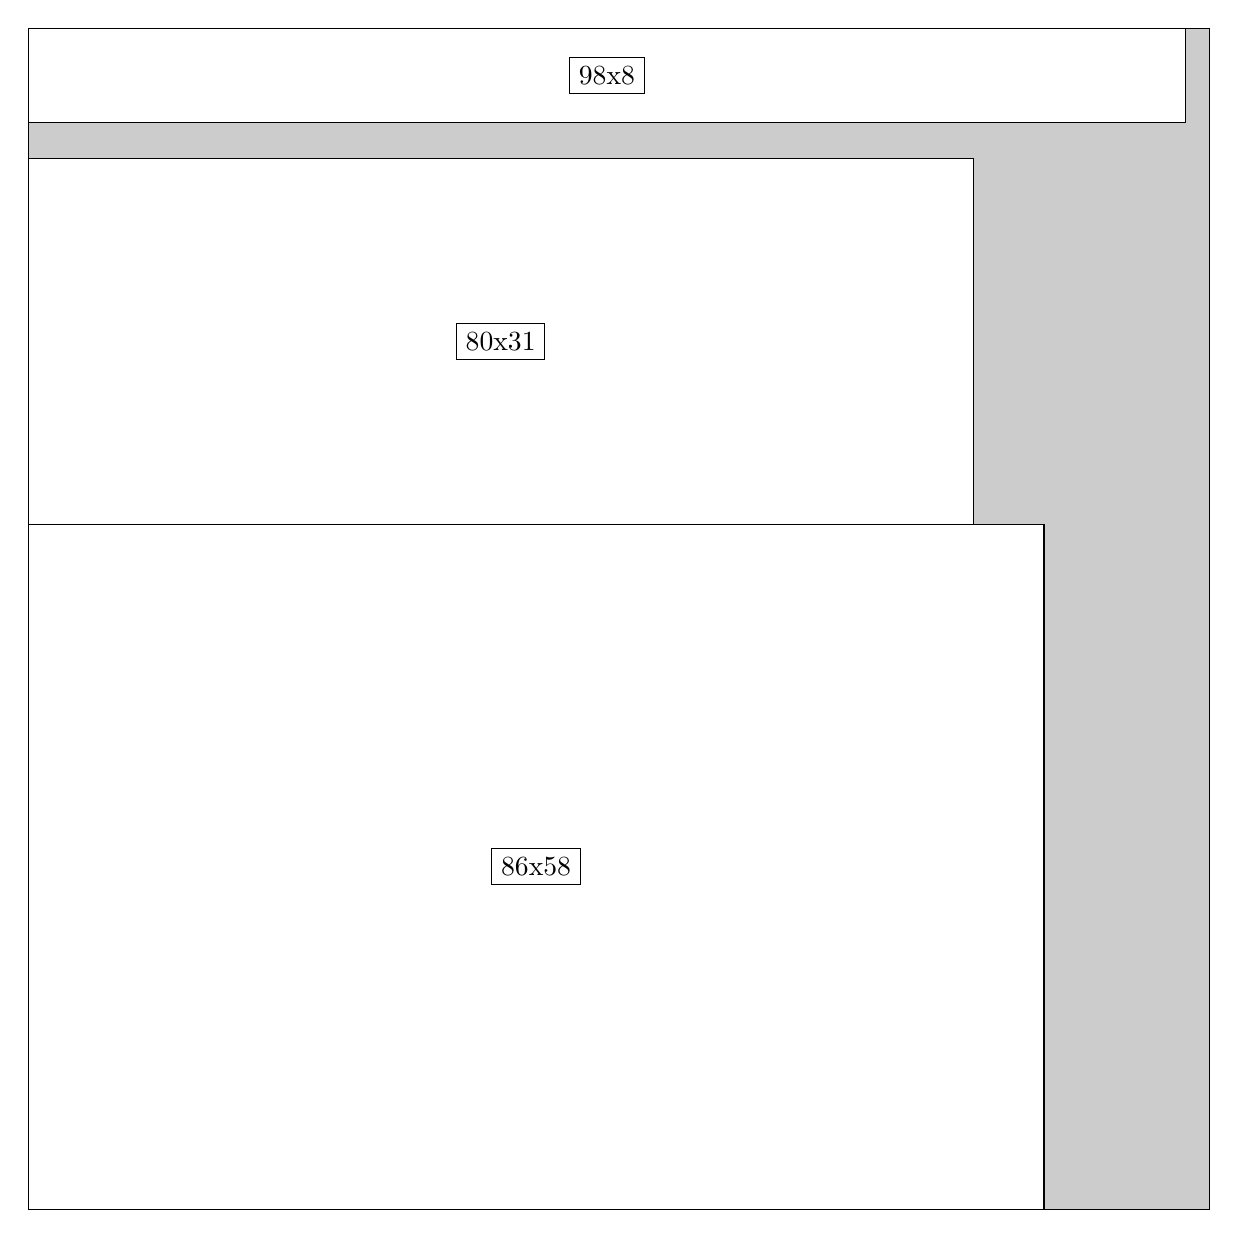
\begin{tikzpicture}[shorten >=1pt,scale=1.0,every node/.style={scale=1.0},->]
\tikzstyle{vertex}=[circle,fill=black!25,minimum size=14pt,inner sep=0pt]
\filldraw[fill=gray!40!white, draw=black] (0,0) rectangle (15.0,15.0);
\foreach \name/\x/\y/\w/\h in {80x31/0.0/8.7/12.0/4.6499999999999995,86x58/0.0/0.0/12.9/8.7,98x8/0.0/13.799999999999999/14.7/1.2}
\filldraw[fill=white!40!white, draw=black] (\x,\y) rectangle node[draw] (\name) {\name} ++(\w,\h);
\end{tikzpicture}


w =80 , h =31 , x =0 , y =58 , v =2480
\par
w =86 , h =58 , x =0 , y =0 , v =4988
\par
w =98 , h =8 , x =0 , y =92 , v =784
\par
\newpage


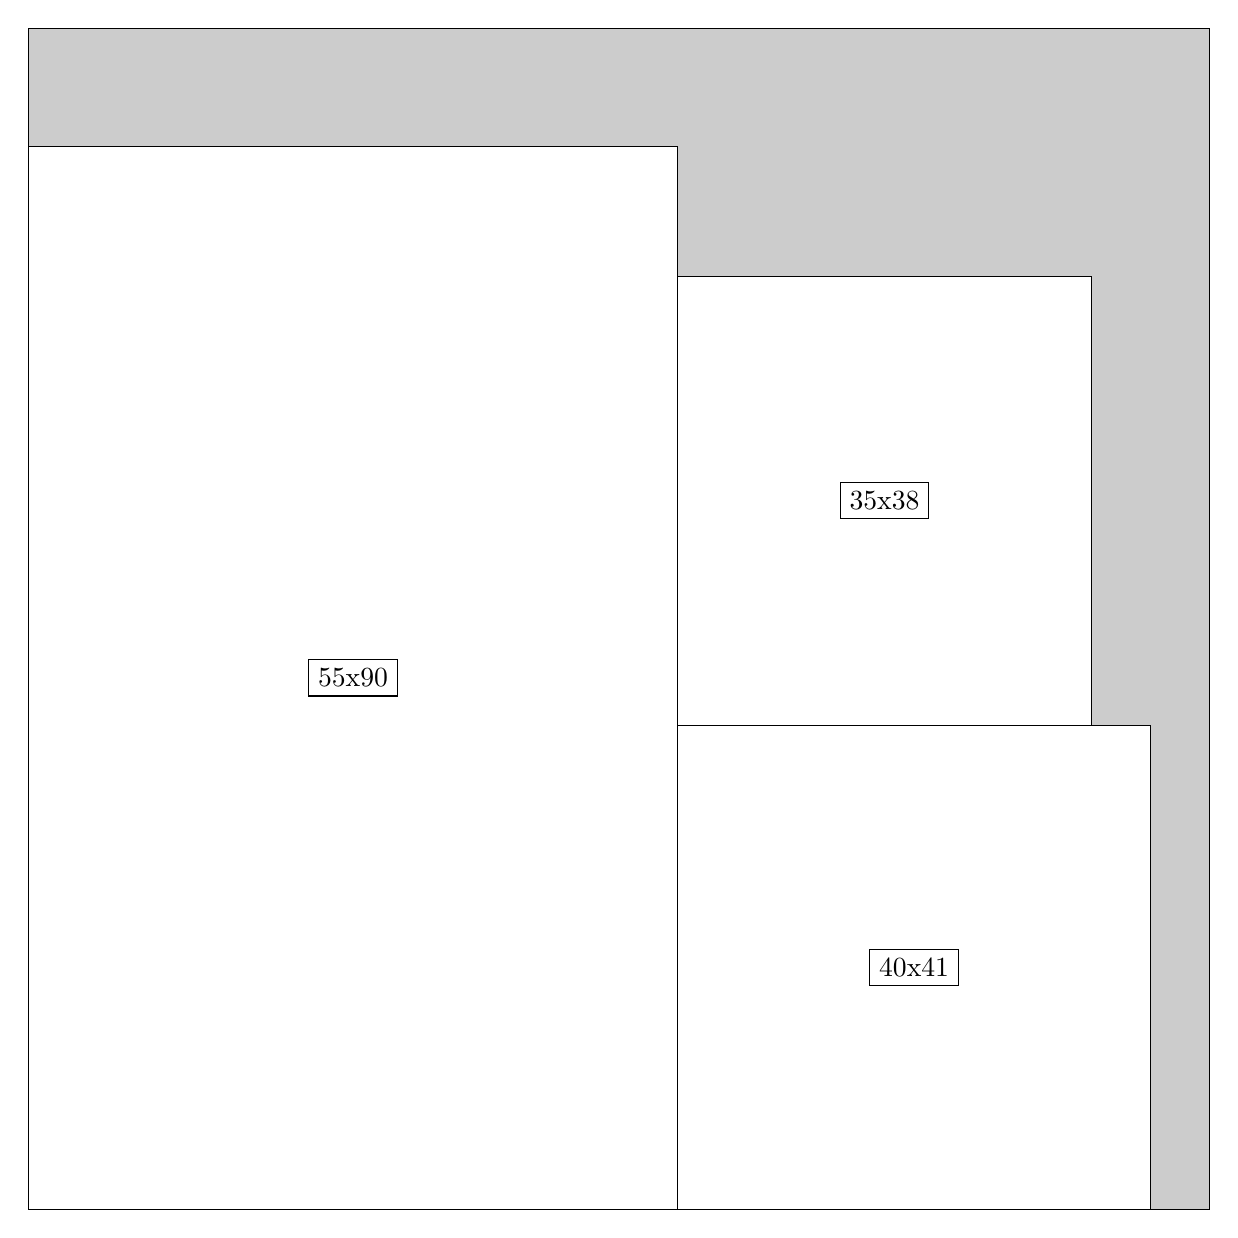
\begin{tikzpicture}[shorten >=1pt,scale=1.0,every node/.style={scale=1.0},->]
\tikzstyle{vertex}=[circle,fill=black!25,minimum size=14pt,inner sep=0pt]
\filldraw[fill=gray!40!white, draw=black] (0,0) rectangle (15.0,15.0);
\foreach \name/\x/\y/\w/\h in {55x90/0.0/0.0/8.25/13.5,40x41/8.25/0.0/6.0/6.1499999999999995,35x38/8.25/6.1499999999999995/5.25/5.7}
\filldraw[fill=white!40!white, draw=black] (\x,\y) rectangle node[draw] (\name) {\name} ++(\w,\h);
\end{tikzpicture}


w =55 , h =90 , x =0 , y =0 , v =4950
\par
w =40 , h =41 , x =55 , y =0 , v =1640
\par
w =35 , h =38 , x =55 , y =41 , v =1330
\par
\newpage


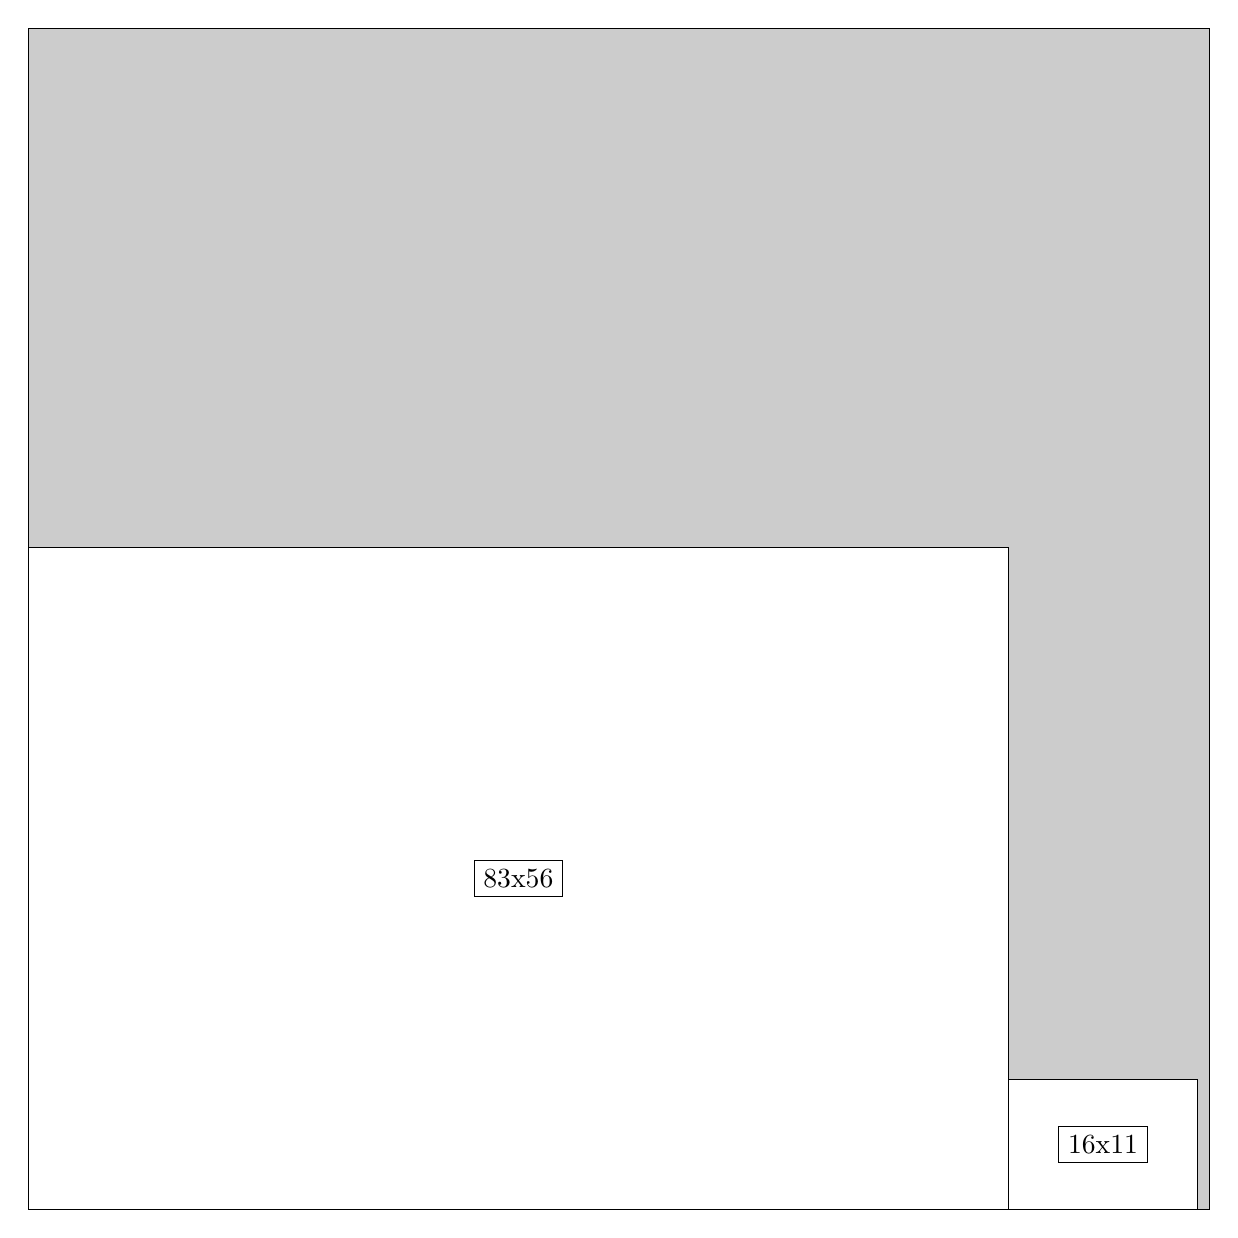
\begin{tikzpicture}[shorten >=1pt,scale=1.0,every node/.style={scale=1.0},->]
\tikzstyle{vertex}=[circle,fill=black!25,minimum size=14pt,inner sep=0pt]
\filldraw[fill=gray!40!white, draw=black] (0,0) rectangle (15.0,15.0);
\foreach \name/\x/\y/\w/\h in {83x56/0.0/0.0/12.45/8.4,16x11/12.45/0.0/2.4/1.65}
\filldraw[fill=white!40!white, draw=black] (\x,\y) rectangle node[draw] (\name) {\name} ++(\w,\h);
\end{tikzpicture}


w =83 , h =56 , x =0 , y =0 , v =4648
\par
w =16 , h =11 , x =83 , y =0 , v =176
\par
\newpage


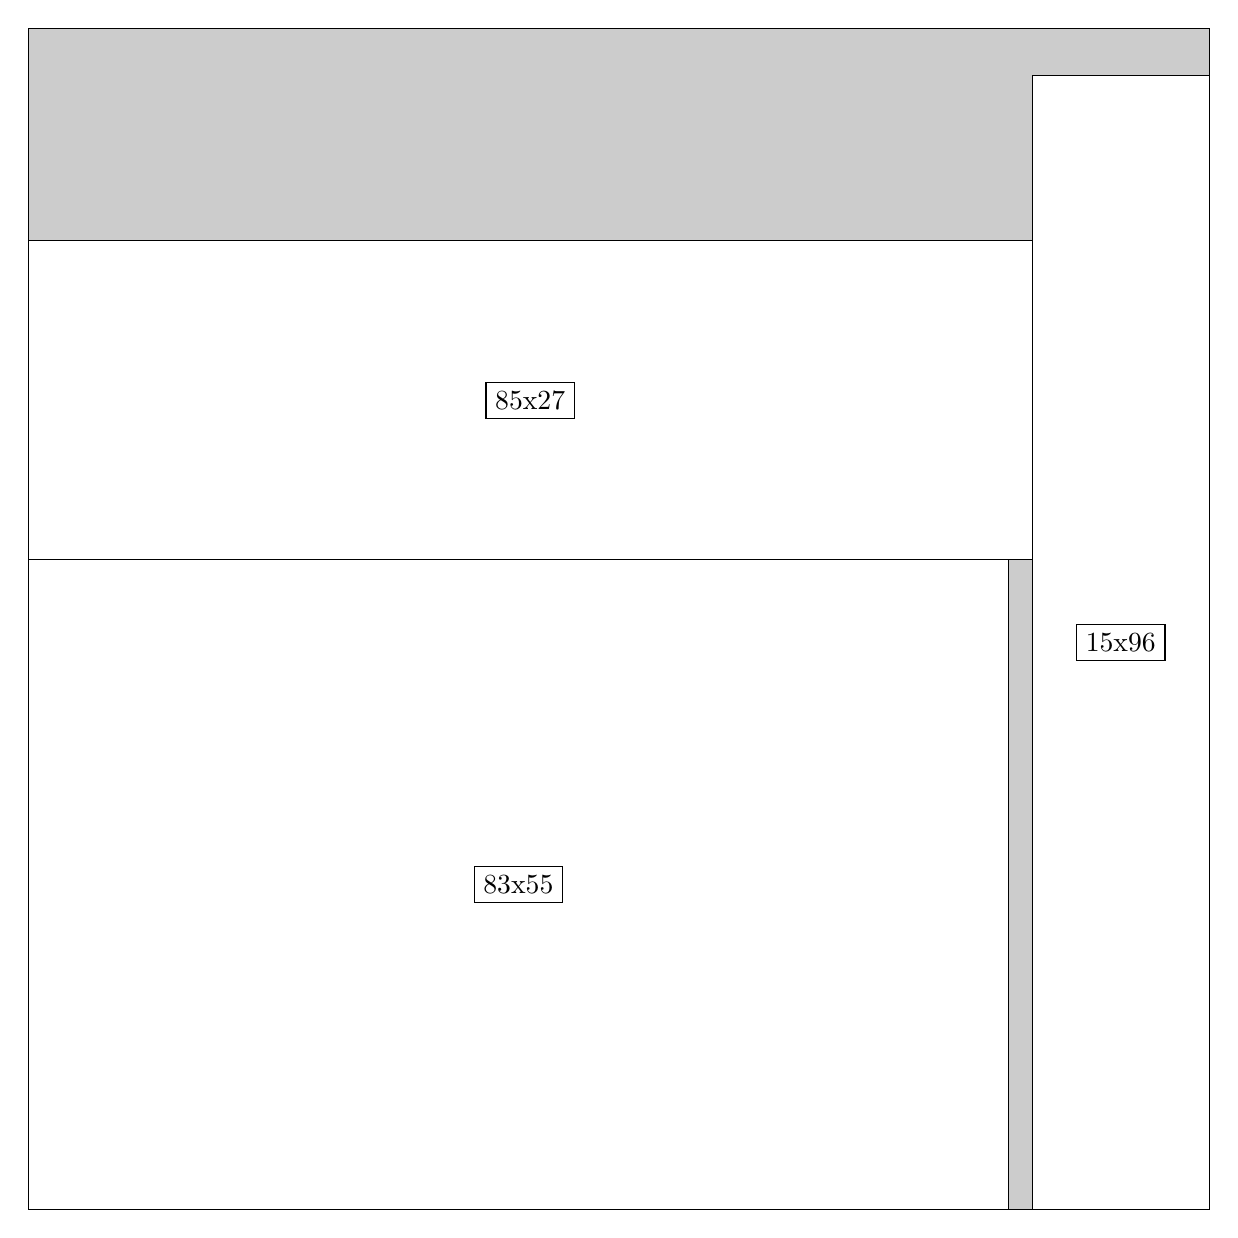
\begin{tikzpicture}[shorten >=1pt,scale=1.0,every node/.style={scale=1.0},->]
\tikzstyle{vertex}=[circle,fill=black!25,minimum size=14pt,inner sep=0pt]
\filldraw[fill=gray!40!white, draw=black] (0,0) rectangle (15.0,15.0);
\foreach \name/\x/\y/\w/\h in {83x55/0.0/0.0/12.45/8.25,85x27/0.0/8.25/12.75/4.05,15x96/12.75/0.0/2.25/14.399999999999999}
\filldraw[fill=white!40!white, draw=black] (\x,\y) rectangle node[draw] (\name) {\name} ++(\w,\h);
\end{tikzpicture}


w =83 , h =55 , x =0 , y =0 , v =4565
\par
w =85 , h =27 , x =0 , y =55 , v =2295
\par
w =15 , h =96 , x =85 , y =0 , v =1440
\par
\newpage


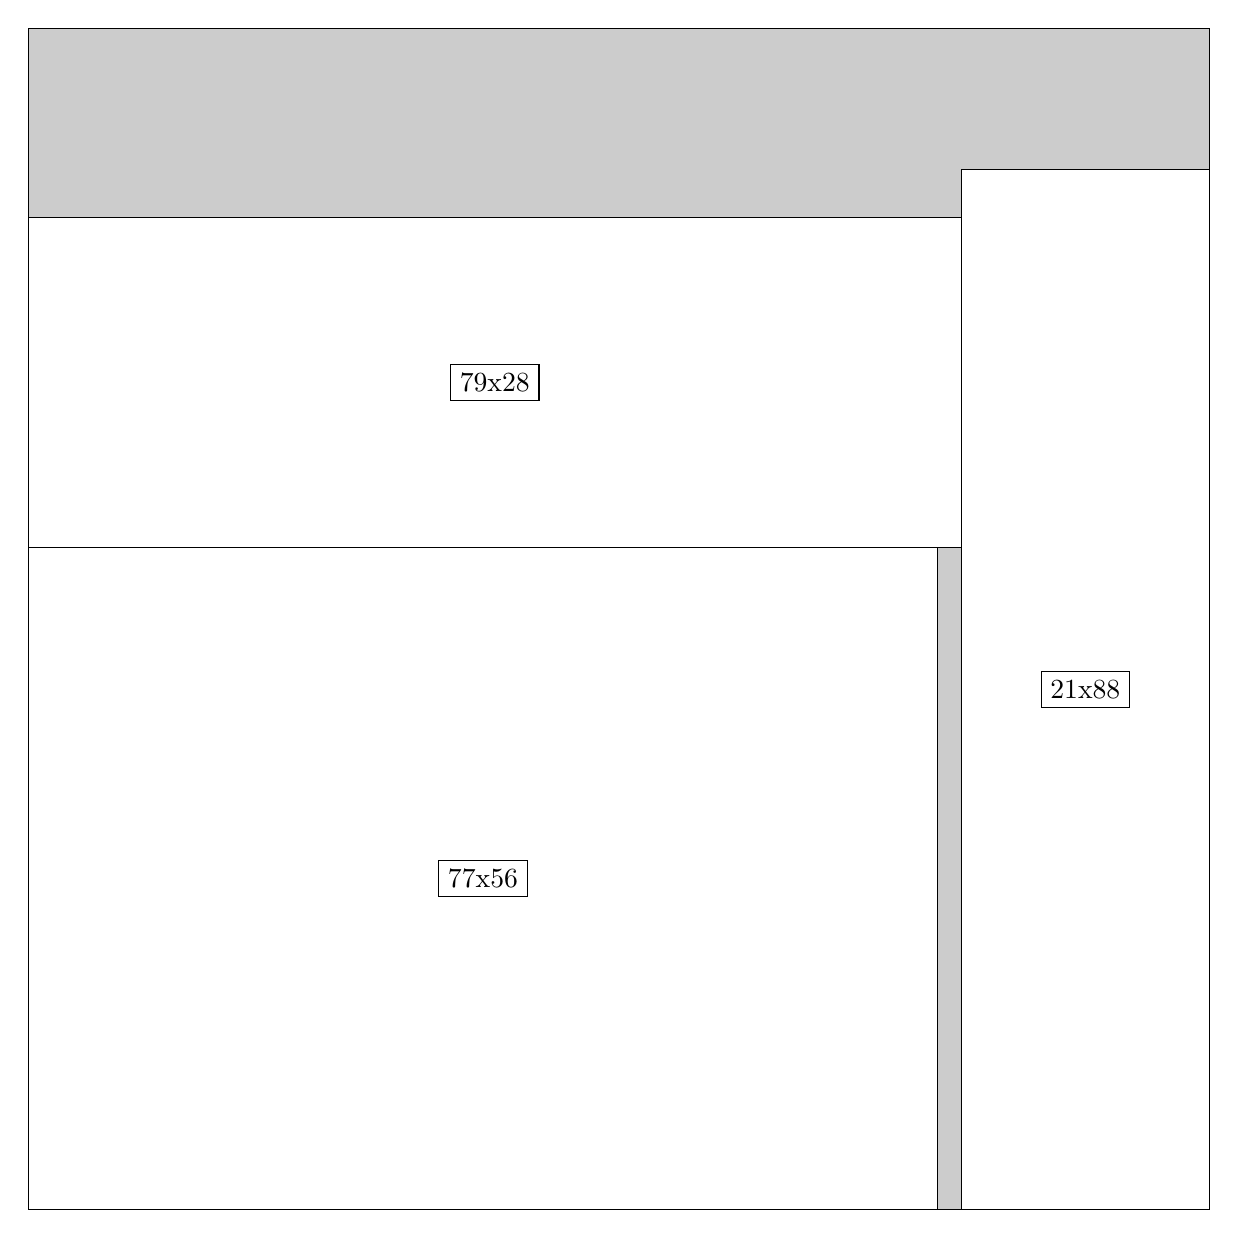
\begin{tikzpicture}[shorten >=1pt,scale=1.0,every node/.style={scale=1.0},->]
\tikzstyle{vertex}=[circle,fill=black!25,minimum size=14pt,inner sep=0pt]
\filldraw[fill=gray!40!white, draw=black] (0,0) rectangle (15.0,15.0);
\foreach \name/\x/\y/\w/\h in {77x56/0.0/0.0/11.549999999999999/8.4,79x28/0.0/8.4/11.85/4.2,21x88/11.85/0.0/3.15/13.2}
\filldraw[fill=white!40!white, draw=black] (\x,\y) rectangle node[draw] (\name) {\name} ++(\w,\h);
\end{tikzpicture}


w =77 , h =56 , x =0 , y =0 , v =4312
\par
w =79 , h =28 , x =0 , y =56 , v =2212
\par
w =21 , h =88 , x =79 , y =0 , v =1848
\par
\newpage


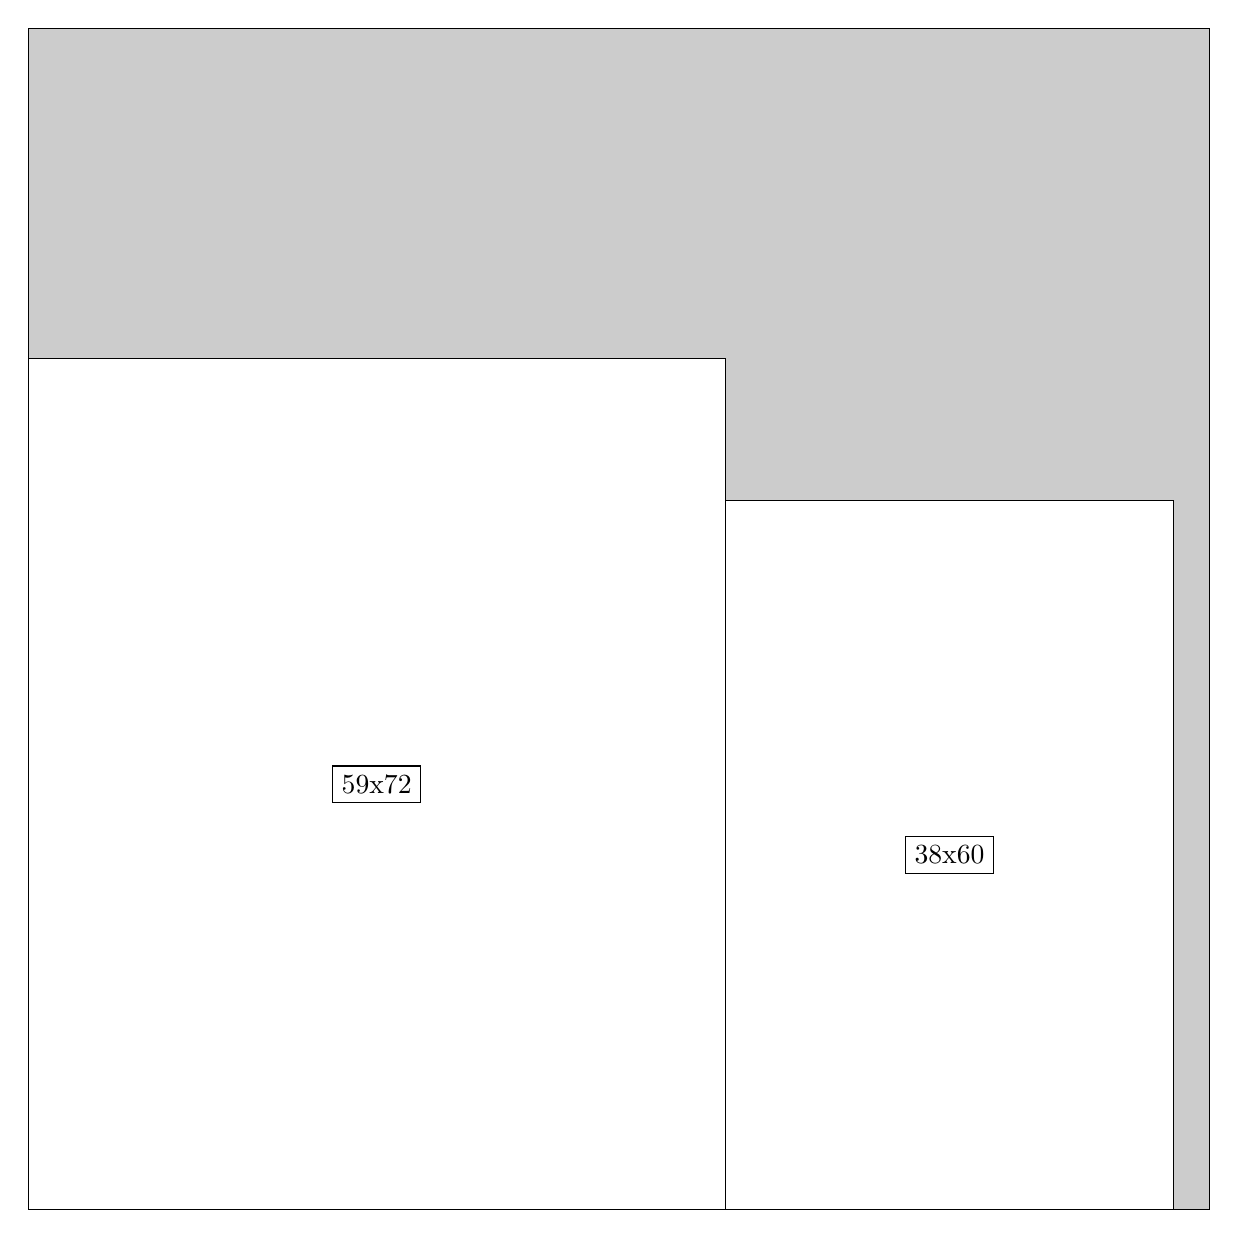
\begin{tikzpicture}[shorten >=1pt,scale=1.0,every node/.style={scale=1.0},->]
\tikzstyle{vertex}=[circle,fill=black!25,minimum size=14pt,inner sep=0pt]
\filldraw[fill=gray!40!white, draw=black] (0,0) rectangle (15.0,15.0);
\foreach \name/\x/\y/\w/\h in {59x72/0.0/0.0/8.85/10.799999999999999,38x60/8.85/0.0/5.7/9.0}
\filldraw[fill=white!40!white, draw=black] (\x,\y) rectangle node[draw] (\name) {\name} ++(\w,\h);
\end{tikzpicture}


w =59 , h =72 , x =0 , y =0 , v =4248
\par
w =38 , h =60 , x =59 , y =0 , v =2280
\par
\newpage


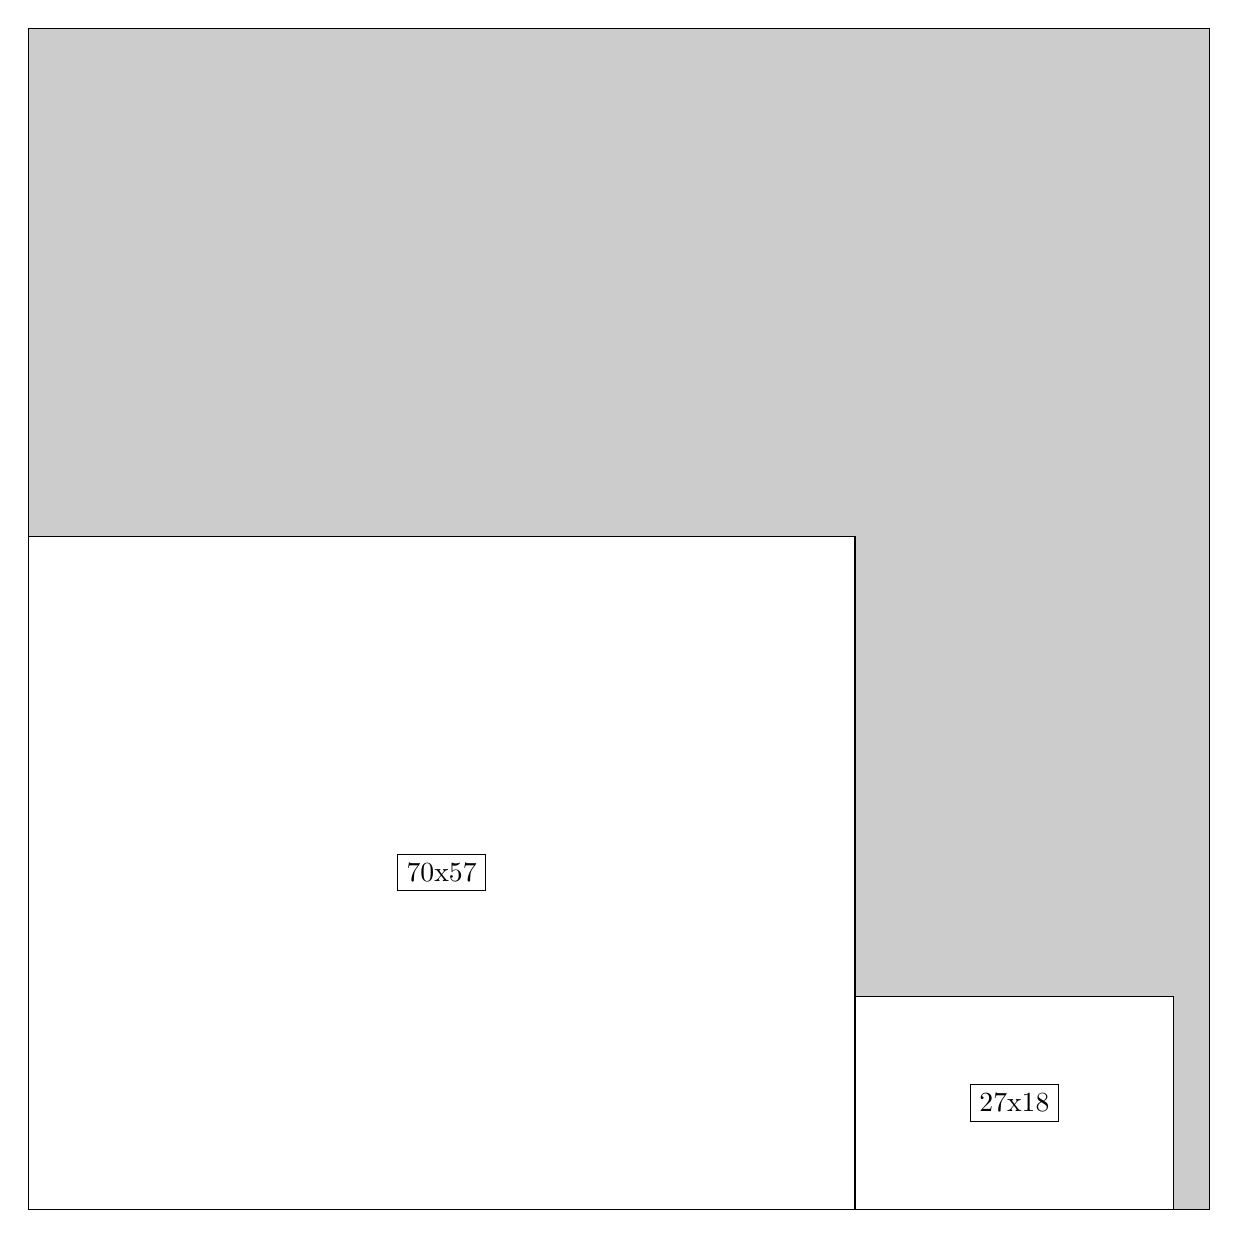
\begin{tikzpicture}[shorten >=1pt,scale=1.0,every node/.style={scale=1.0},->]
\tikzstyle{vertex}=[circle,fill=black!25,minimum size=14pt,inner sep=0pt]
\filldraw[fill=gray!40!white, draw=black] (0,0) rectangle (15.0,15.0);
\foreach \name/\x/\y/\w/\h in {70x57/0.0/0.0/10.5/8.549999999999999,27x18/10.5/0.0/4.05/2.6999999999999997}
\filldraw[fill=white!40!white, draw=black] (\x,\y) rectangle node[draw] (\name) {\name} ++(\w,\h);
\end{tikzpicture}


w =70 , h =57 , x =0 , y =0 , v =3990
\par
w =27 , h =18 , x =70 , y =0 , v =486
\par
\newpage


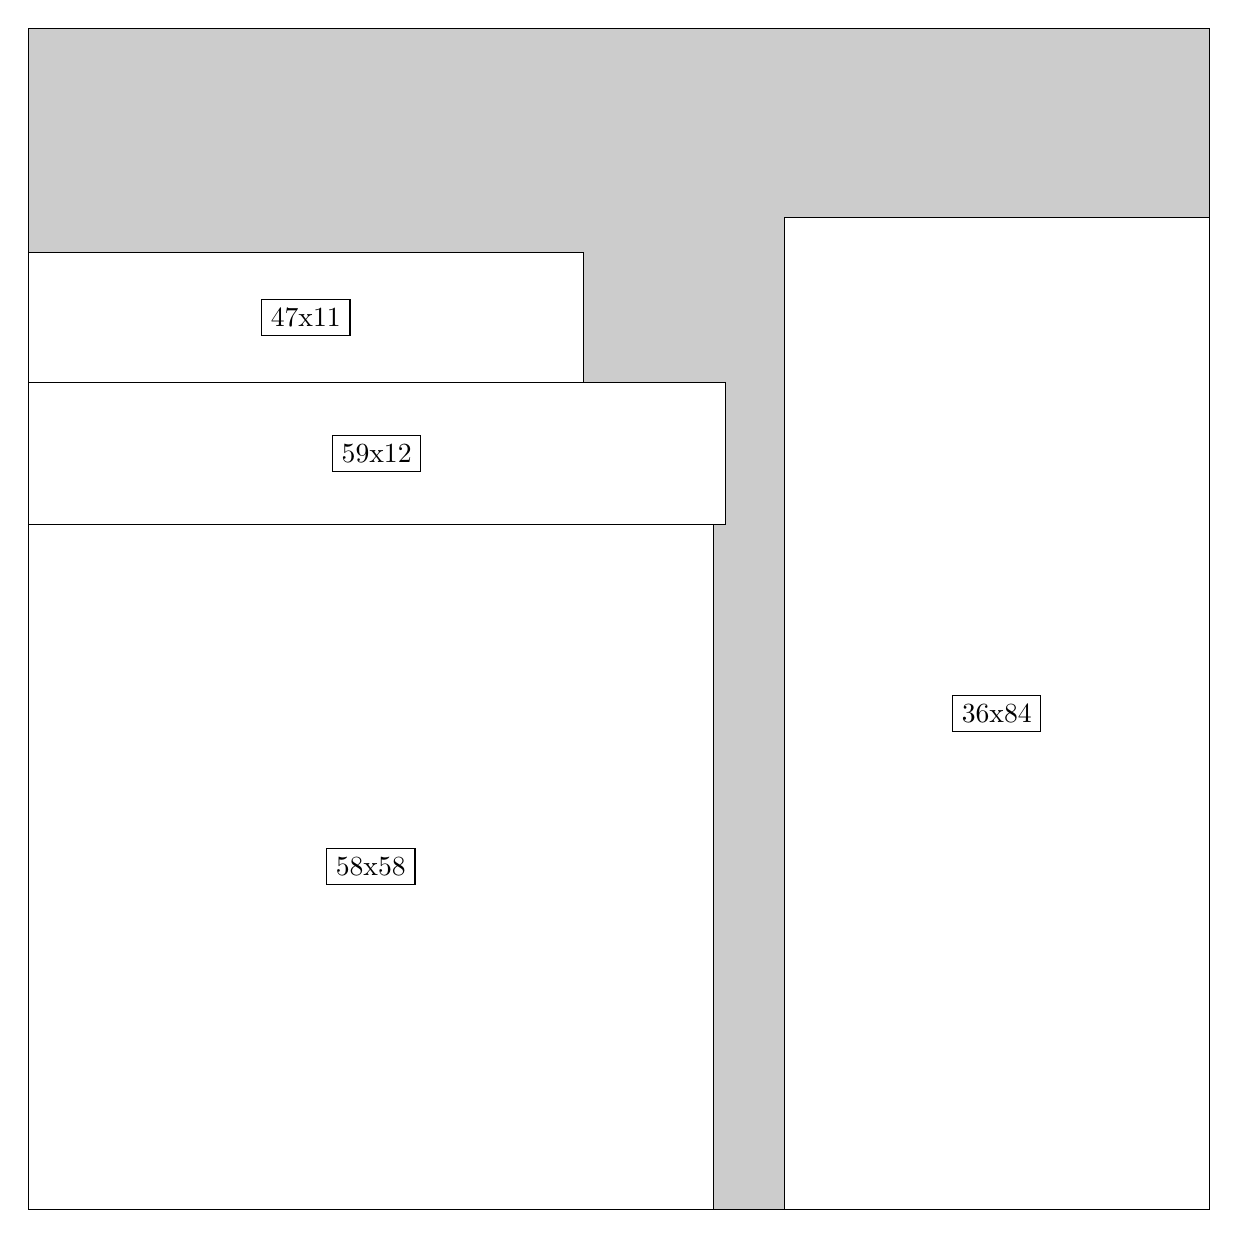
\begin{tikzpicture}[shorten >=1pt,scale=1.0,every node/.style={scale=1.0},->]
\tikzstyle{vertex}=[circle,fill=black!25,minimum size=14pt,inner sep=0pt]
\filldraw[fill=gray!40!white, draw=black] (0,0) rectangle (15.0,15.0);
\foreach \name/\x/\y/\w/\h in {58x58/0.0/0.0/8.7/8.7,36x84/9.6/0.0/5.3999999999999995/12.6,59x12/0.0/8.7/8.85/1.7999999999999998,47x11/0.0/10.5/7.05/1.65}
\filldraw[fill=white!40!white, draw=black] (\x,\y) rectangle node[draw] (\name) {\name} ++(\w,\h);
\end{tikzpicture}


w =58 , h =58 , x =0 , y =0 , v =3364
\par
w =36 , h =84 , x =64 , y =0 , v =3024
\par
w =59 , h =12 , x =0 , y =58 , v =708
\par
w =47 , h =11 , x =0 , y =70 , v =517
\par
\newpage


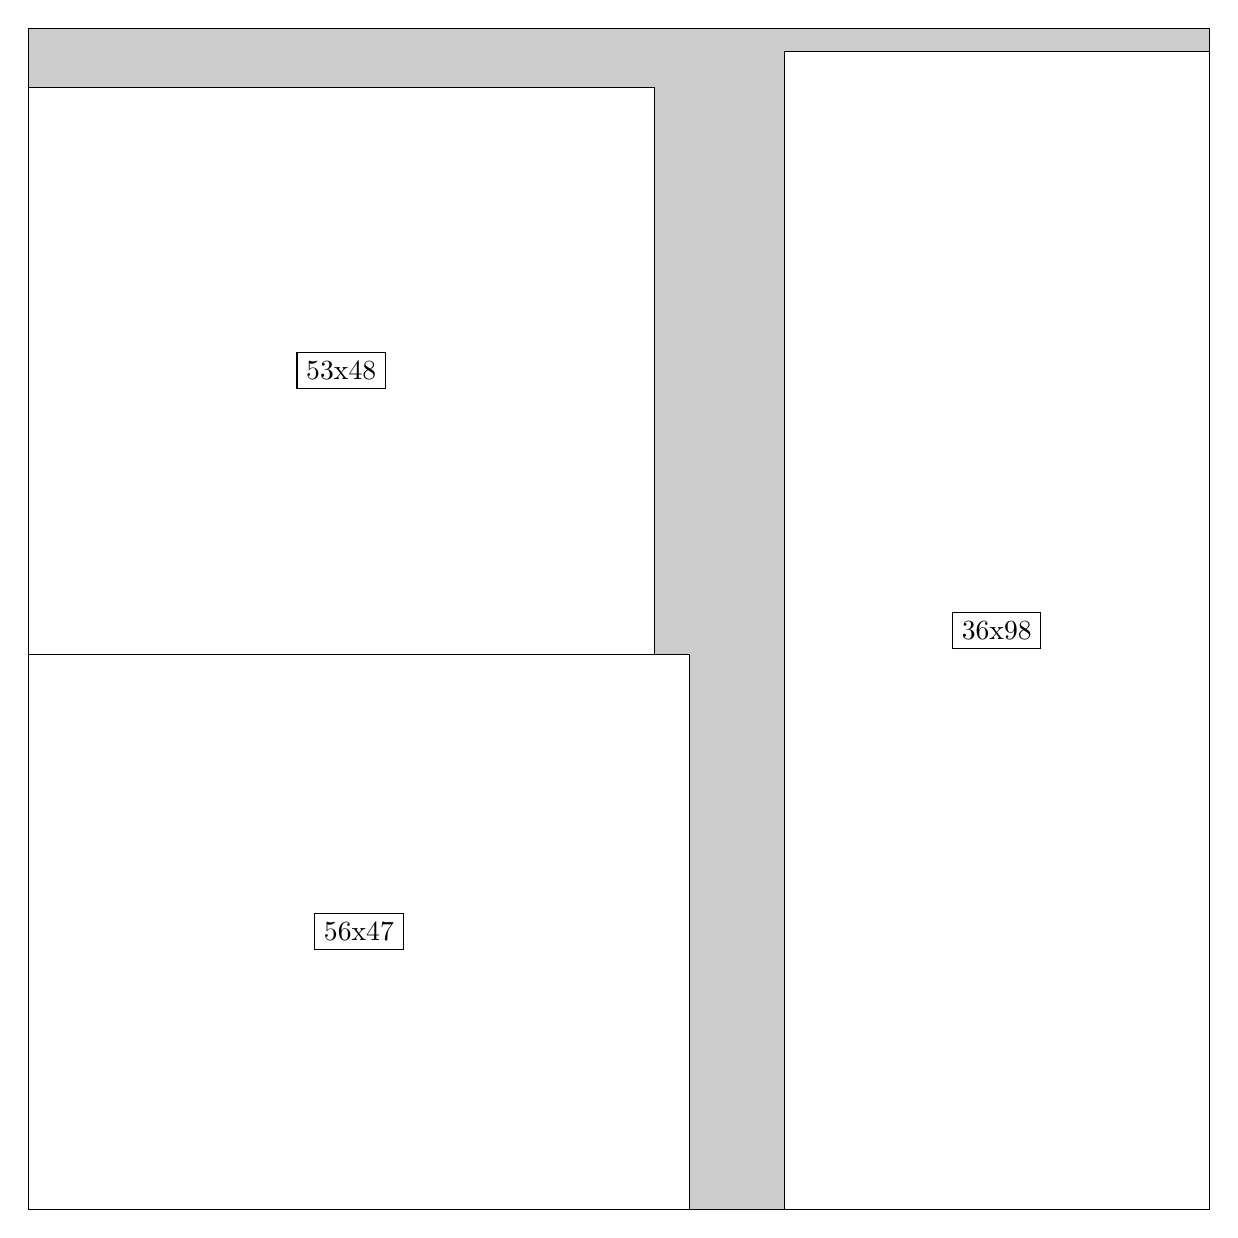
\begin{tikzpicture}[shorten >=1pt,scale=1.0,every node/.style={scale=1.0},->]
\tikzstyle{vertex}=[circle,fill=black!25,minimum size=14pt,inner sep=0pt]
\filldraw[fill=gray!40!white, draw=black] (0,0) rectangle (15.0,15.0);
\foreach \name/\x/\y/\w/\h in {36x98/9.6/0.0/5.3999999999999995/14.7,56x47/0.0/0.0/8.4/7.05,53x48/0.0/7.05/7.949999999999999/7.199999999999999}
\filldraw[fill=white!40!white, draw=black] (\x,\y) rectangle node[draw] (\name) {\name} ++(\w,\h);
\end{tikzpicture}


w =36 , h =98 , x =64 , y =0 , v =3528
\par
w =56 , h =47 , x =0 , y =0 , v =2632
\par
w =53 , h =48 , x =0 , y =47 , v =2544
\par
\newpage


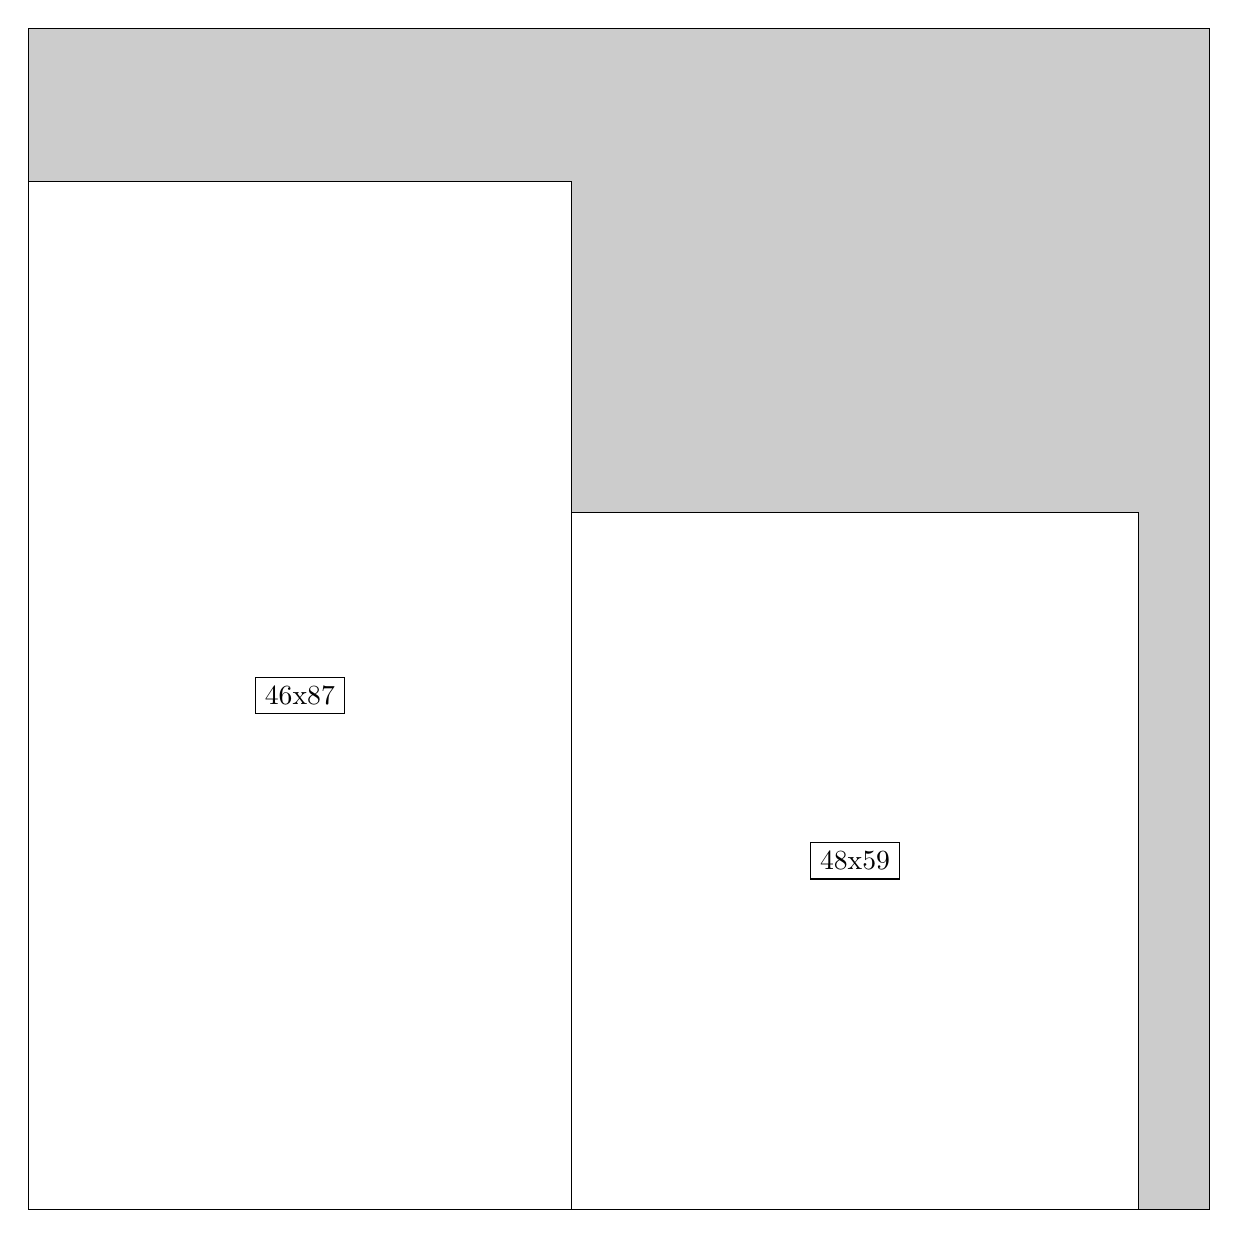
\begin{tikzpicture}[shorten >=1pt,scale=1.0,every node/.style={scale=1.0},->]
\tikzstyle{vertex}=[circle,fill=black!25,minimum size=14pt,inner sep=0pt]
\filldraw[fill=gray!40!white, draw=black] (0,0) rectangle (15.0,15.0);
\foreach \name/\x/\y/\w/\h in {46x87/0.0/0.0/6.8999999999999995/13.049999999999999,48x59/6.8999999999999995/0.0/7.199999999999999/8.85}
\filldraw[fill=white!40!white, draw=black] (\x,\y) rectangle node[draw] (\name) {\name} ++(\w,\h);
\end{tikzpicture}


w =46 , h =87 , x =0 , y =0 , v =4002
\par
w =48 , h =59 , x =46 , y =0 , v =2832
\par
\newpage


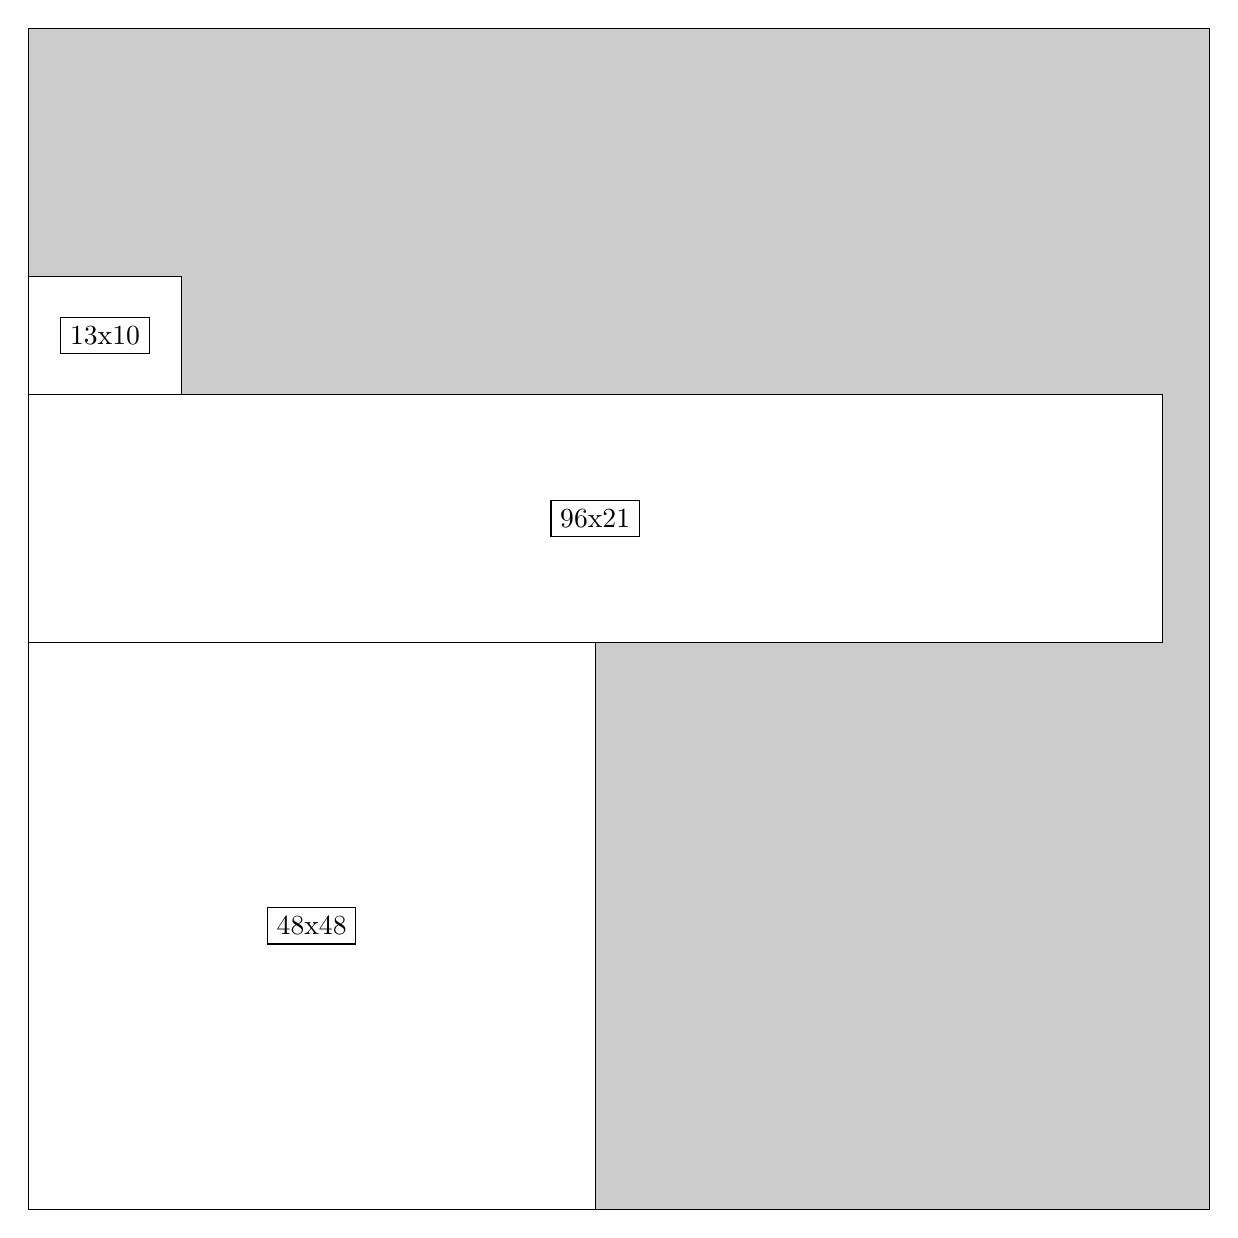
\begin{tikzpicture}[shorten >=1pt,scale=1.0,every node/.style={scale=1.0},->]
\tikzstyle{vertex}=[circle,fill=black!25,minimum size=14pt,inner sep=0pt]
\filldraw[fill=gray!40!white, draw=black] (0,0) rectangle (15.0,15.0);
\foreach \name/\x/\y/\w/\h in {48x48/0.0/0.0/7.199999999999999/7.199999999999999,96x21/0.0/7.199999999999999/14.399999999999999/3.15,13x10/0.0/10.35/1.95/1.5}
\filldraw[fill=white!40!white, draw=black] (\x,\y) rectangle node[draw] (\name) {\name} ++(\w,\h);
\end{tikzpicture}


w =48 , h =48 , x =0 , y =0 , v =2304
\par
w =96 , h =21 , x =0 , y =48 , v =2016
\par
w =13 , h =10 , x =0 , y =69 , v =130
\par
\newpage


\end{document}